% 2026-10-23：按学习复现、探索尝试、优化验证、迭代调试、整板尝试重组。
\documentclass[stage2,fontset=fandol]{ydzjreport}
\usepackage{subcaption,longtable}
\usepackage{bm}
\stagetwosetup
{第 3 个逻辑月 · 优化与验证}
{冯旭东、陈思文、张昊洋}
{复合微通道分区冷却}
{【待确认】逻辑月 3 对应的自然月}
{翼型专题；参数分组；UDF 修改；网格检验；PID 数学模拟}
{细化翼型参数研究，整理既有翼型结果与待补分组方案；修改并核验 UDF，分析网格敏感性，并开展纯数学温控模拟。}
\pagestyle{empty}   % 去掉页眉与页脚（含页码）
\RemoveFromHook{enddocument}[ydzjreport] % 去掉末页的作者与格式规范收尾说明


\newlabel{eq:newton}{{1}{4}{翼型差异的定性机理解释}{equation.2.1}{}}
\newlabel{eq:nu}{{2}{4}{翼型差异的定性机理解释}{equation.2.2}{}}
\newlabel{eq:friction}{{3}{4}{翼型差异的定性机理解释}{equation.2.3}{}}
\newlabel{eq:pec}{{4}{5}{翼型差异的定性机理解释}{equation.2.4}{}}
\newlabel{eq:adverse}{{5}{5}{翼型差异的定性机理解释}{equation.2.5}{}}
\newlabel{eq:shear}{{6}{5}{翼型差异的定性机理解释}{equation.2.6}{}}
\newlabel{eq:hgrad}{{7}{5}{翼型差异的定性机理解释}{equation.2.7}{}}
\newlabel{eq:mesh_error}{{9}{8}{统一比较条件与误差定义。}{equation.2.9}{}}
\newlabel{eq:pid}{{10}{14}{初步数学模型与最小闭环验证}{equation.2.10}{}}
\begin{document}
\section*{逻辑月3\_形态与物理：图表附件}
本附件图表编号与对应提交正文及完整报告一致。\par\clearpage
\setcounter{table}{0}
\begin{table}[H]\centering
\small
\renewcommand{\arraystretch}{1.12}
\caption{翼型扰流柱的参数体系与变量取值方式}\label{tab:param-vars}
\begin{tabularx}{\textwidth}{@{}>{\RaggedRight\arraybackslash}p{0.20\textwidth} Y Y@{}}
\toprule
\rowcolor{ydzjlight} 参数类别 & 参数 & 定义与取值方式 \\
\midrule
结构几何参数（翼型主体） & 弦长 & 基础几何量，长度量纲；其余位置类参数以其无量纲化为基准 \\[3pt]
& 柱高 & 基础几何量，长度量纲，决定扰流柱在通道内的高度 \\[3pt]
& 迎角 & 基础几何量，角度量纲；统一表征来流方向，不另设来流方向变量 \\[3pt]
& 弯度幅值 & 核心调控量，随机取值，用于生成差异化的翼型基准构型 \\[3pt]
& 弯度弦向位置 & 核心调控量，以弦长方向的无量纲比例定义，随机取值 \\[3pt]
& 厚度幅值 & 核心调控量，随机取值，与弯度幅值共同决定基准剖面形态 \\[3pt]
& 厚度弦向位置 & 核心调控量，以弦长方向的无量纲比例定义，随机取值 \\[3pt]
\midrule
结构几何参数（尾部构型） & 尾部段长度 & 尾缘段沿弦向的延伸长度，长度量纲 \\[3pt]
& 尾部截面长宽比 & 尾部截面几何比例，无量纲 \\[3pt]
& 尾部上下段长度比 & 尾部经中线截断后上、下两段长度之比，无量纲 \\[3pt]
& 尾部过渡连接方式 & 采用形函数平滑过渡，在幂函数、余弦函数、正弦幂函数、指数函数四类候选函数中选型 \\[3pt]
\midrule
外部运行参数 & 来流速度 & 唯一可调的运行变量 \\[3pt]
& 来流方向 & 已纳入迎角参数统一表征，不单列 \\[3pt]
& 入口温度 & 固定边界条件，取定值，不纳入优化变量范围 \\[3pt]
& 加热温度 & 固定边界条件，取定值，不纳入优化变量范围 \\[3pt]
\bottomrule\end{tabularx}\end{table}
\clearpage
\setcounter{table}{1}
\begin{table}[H]
\centering
\caption{不同翼型构型流热耦合仿真关键结果（基准工况）}
\label{tab:airfoil}
\begin{tabularx}{\textwidth}{@{}l c c c c@{}}
\toprule
\rowcolor{ydzjlight} 构型 & 最高温度 / K & 底板平均温度 / K & $h$ / (W/(m$^2$·K)) & PEC \\
\midrule
NACA0015 & 357.9 & 356.1 & 756.6 & 1.00 \\
NACA0021 & 355.7 & 354.0 & 765.3 & 1.10 \\
NACA0024 & 354.9 & 353.2 & 798.5 & 1.19 \\
NACA4424 & 354.4 & 352.7 & 789.8 & 1.21 \\
NACA6424 & 358.1 & 356.3 & 750.5 & 1.00 \\
NACA6624 & 357.9 & 356.1 & 750.2 & 1.01 \\
\bottomrule
\end{tabularx}
\end{table}
\clearpage
\setcounter{table}{2}
\begin{longtable}{@{}r p{0.30\textwidth} r r r r@{}}
\caption{翼型小模型的温度及水力性能汇总（按数据来源与工况分组）}
\label{tab:results}\\
\toprule
\rowcolor{ydzjlight} 热流密度 & 模型或分支 & 最高温度 & 平均温度 & 压差 & 水力功率 \\
/ (W/cm$^2$) & & / $^\circ$C & / $^\circ$C & / kPa & / W \\
\midrule
\endfirsthead
\caption[]{翼型小模型的温度及水力性能汇总（续）}\\
\toprule
\rowcolor{ydzjlight} 热流密度 & 模型或分支 & 最高温度 & 平均温度 & 压差 & 水力功率 \\
/ (W/cm$^2$) & & / $^\circ$C & / $^\circ$C & / kPa & / W \\
\midrule
\endhead
\midrule
\multicolumn{6}{r}{\small 接下页}\\
\endfoot
\bottomrule
\endlastfoot
\multicolumn{6}{@{}l@{}}{\textbf{NACA 小模型：350 W/cm$^2$}}\\
350.00 & 0016 A06 基础 & 58.20 & 34.18 & 3.393 & 0.05428 \\
350.00 & 2416 A00 core & 71.03 & 40.07 & 2.456 & 0.03929 \\
350.00 & 2416 A00 尾部 BOI & 71.01 & 39.25 & 2.512 & 0.04019 \\
350.00 & 0016 A06 拟合物性 & 59.61 & 34.62 & 4.290 & 0.06864 \\
350.00 & 0016 A06 REFPROP & 59.54 & 34.59 & 4.290 & 0.06864 \\
350.00 & 2416 v3 & 72.83 & 38.74 & 2.348 & 0.03757 \\
\midrule
\multicolumn{6}{@{}l@{}}{\textbf{NACA v2 小模型：450 W/cm$^2$}}\\
450.00 & NACA0016 v2 & 85.34 & 43.21 & 2.248 & 0.03596 \\
450.00 & NACA1416 v2 & 85.31 & 43.46 & 2.255 & 0.03609 \\
450.00 & NACA3416 v2 & 85.11 & 43.12 & 2.366 & 0.03785 \\
\midrule
\multicolumn{6}{@{}l@{}}{\textbf{NACA2420：1 s 时刻的瞬时热流密度}}\\
126.82 & 2420 v4 原始 & 43.08 & 31.40 & 1.377 & 0.01653 \\
126.82 & 2420 回流 300 K & 44.23 & 31.83 & 1.651 & 0.01988 \\
126.82 & 2420 IAPWS $\Delta t=0.01$ s & 44.32 & 31.87 & 1.652 & 0.01989 \\
126.82 & 2420 IAPWS $\Delta t=0.005$ s & 44.32 & 31.87 & 1.652 & 0.01989 \\
\end{longtable}
\clearpage
\setcounter{figure}{0}
\begin{figure}[H]
\centering
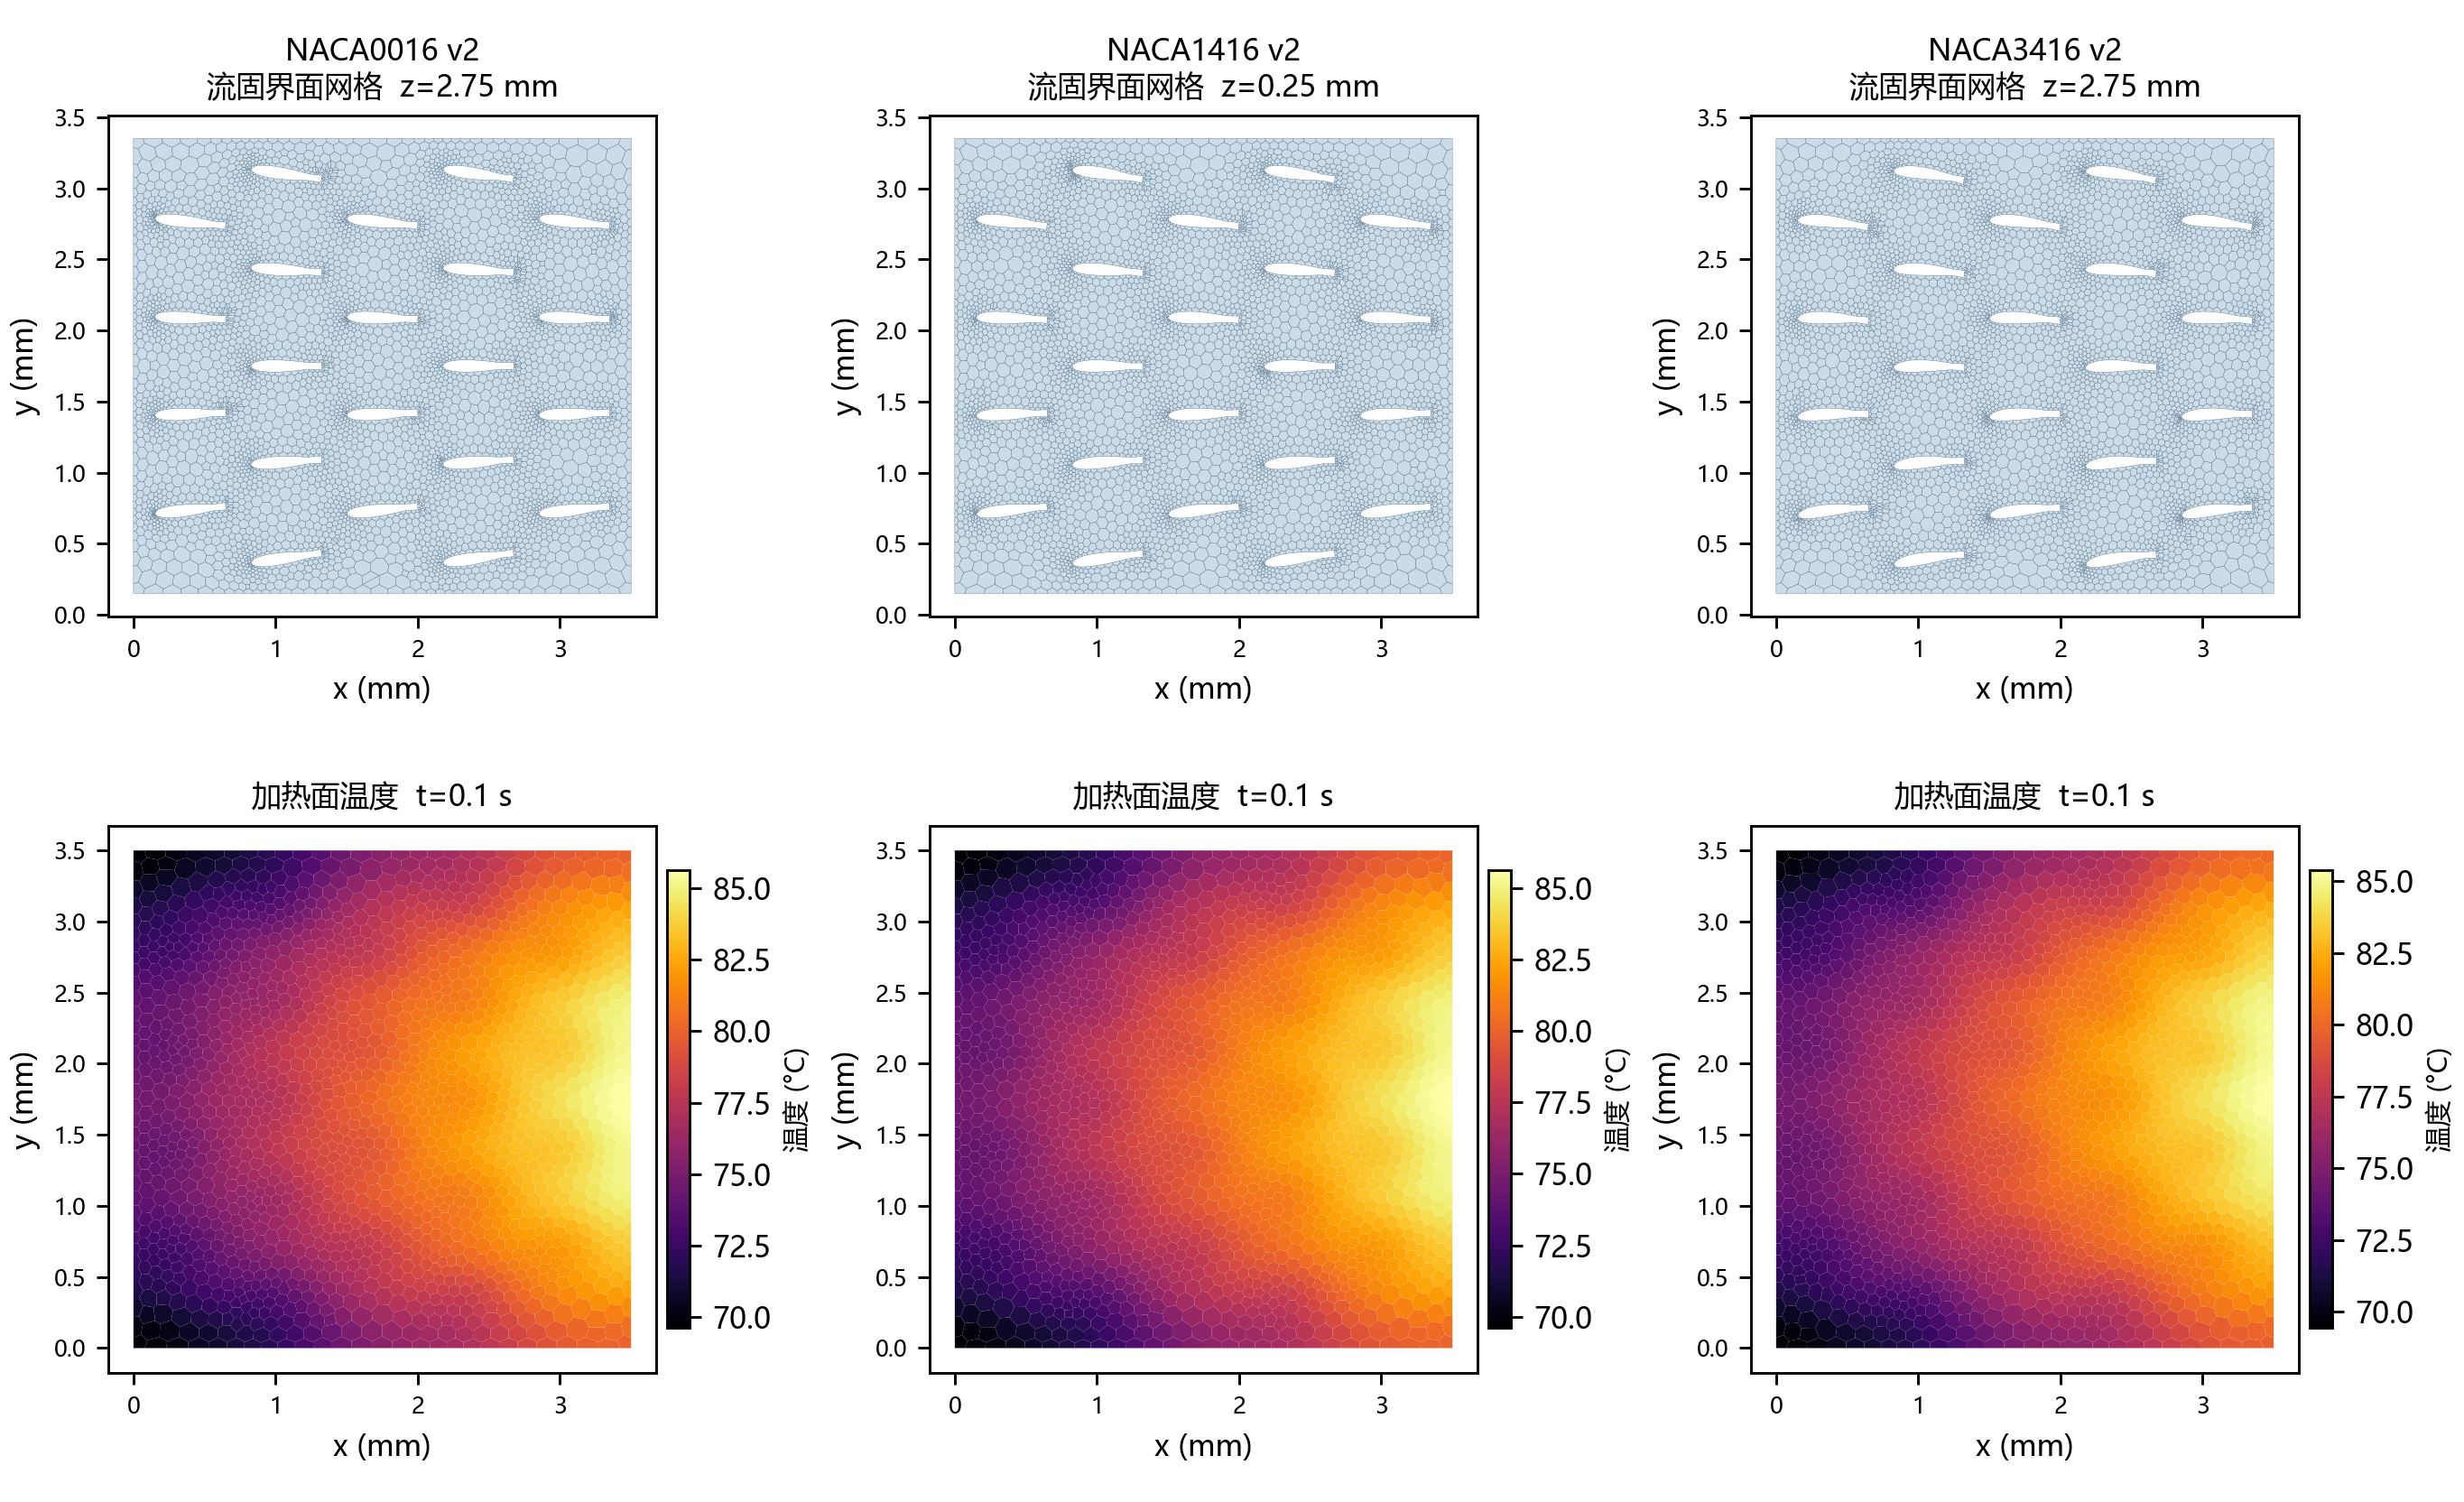
\includegraphics[width=\textwidth]{../../figs/month2_naca_models.png}
\caption{NACA0016、1416、3416 v2 小模型的界面网格与 0.10 s 加热面温度。上排为实际平面流固界面网格，下排温度来自各自配套 Data 文件，色标独立。}
\label{fig:naca-small}
\end{figure}
\clearpage
\setcounter{figure}{1}
\begin{figure}[htbp]\centering
\begin{subfigure}[t]{.49\linewidth}\centering
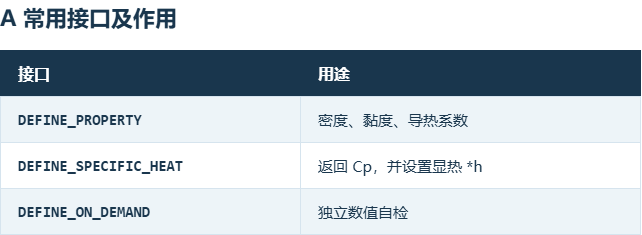
\includegraphics[width=\linewidth]{../../figs/udf_learning_interfaces_a.png}
\caption{常用接口及作用}
\end{subfigure}\hfill
\begin{subfigure}[t]{.49\linewidth}\centering
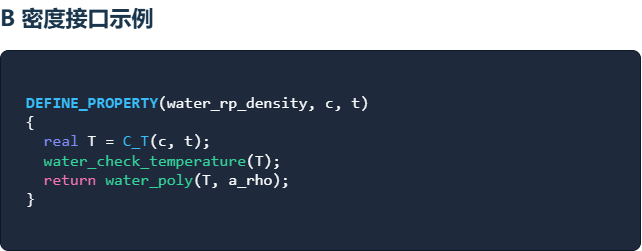
\includegraphics[width=\linewidth]{../../figs/udf_learning_interfaces_b.png}
\caption{密度接口示例}
\end{subfigure}

\vspace{3mm}
\begin{subfigure}[t]{.49\linewidth}\centering
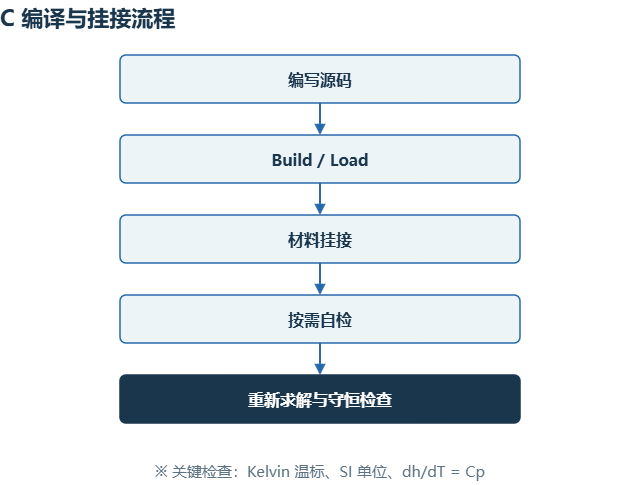
\includegraphics[width=\linewidth]{../../figs/udf_learning_interfaces_c.png}
\caption{编译与挂接流程}
\end{subfigure}\hfill
\begin{subfigure}[t]{.49\linewidth}\centering
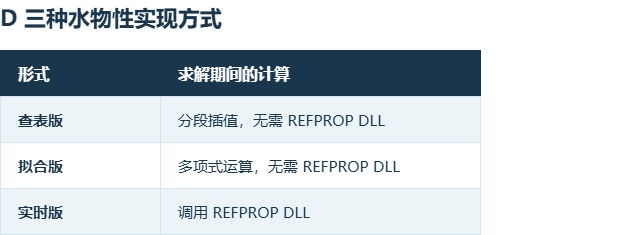
\includegraphics[width=\linewidth]{../../figs/udf_learning_interfaces_d.png}
\caption{三种水物性实现方式}
\end{subfigure}
\caption{水物性 UDF 的接口与实现流程；作为本月修改和核验的方法说明。}\label{fig:udf-interfaces}
\end{figure}
\clearpage
\setcounter{figure}{2}
\begin{figure}[htbp]\centering
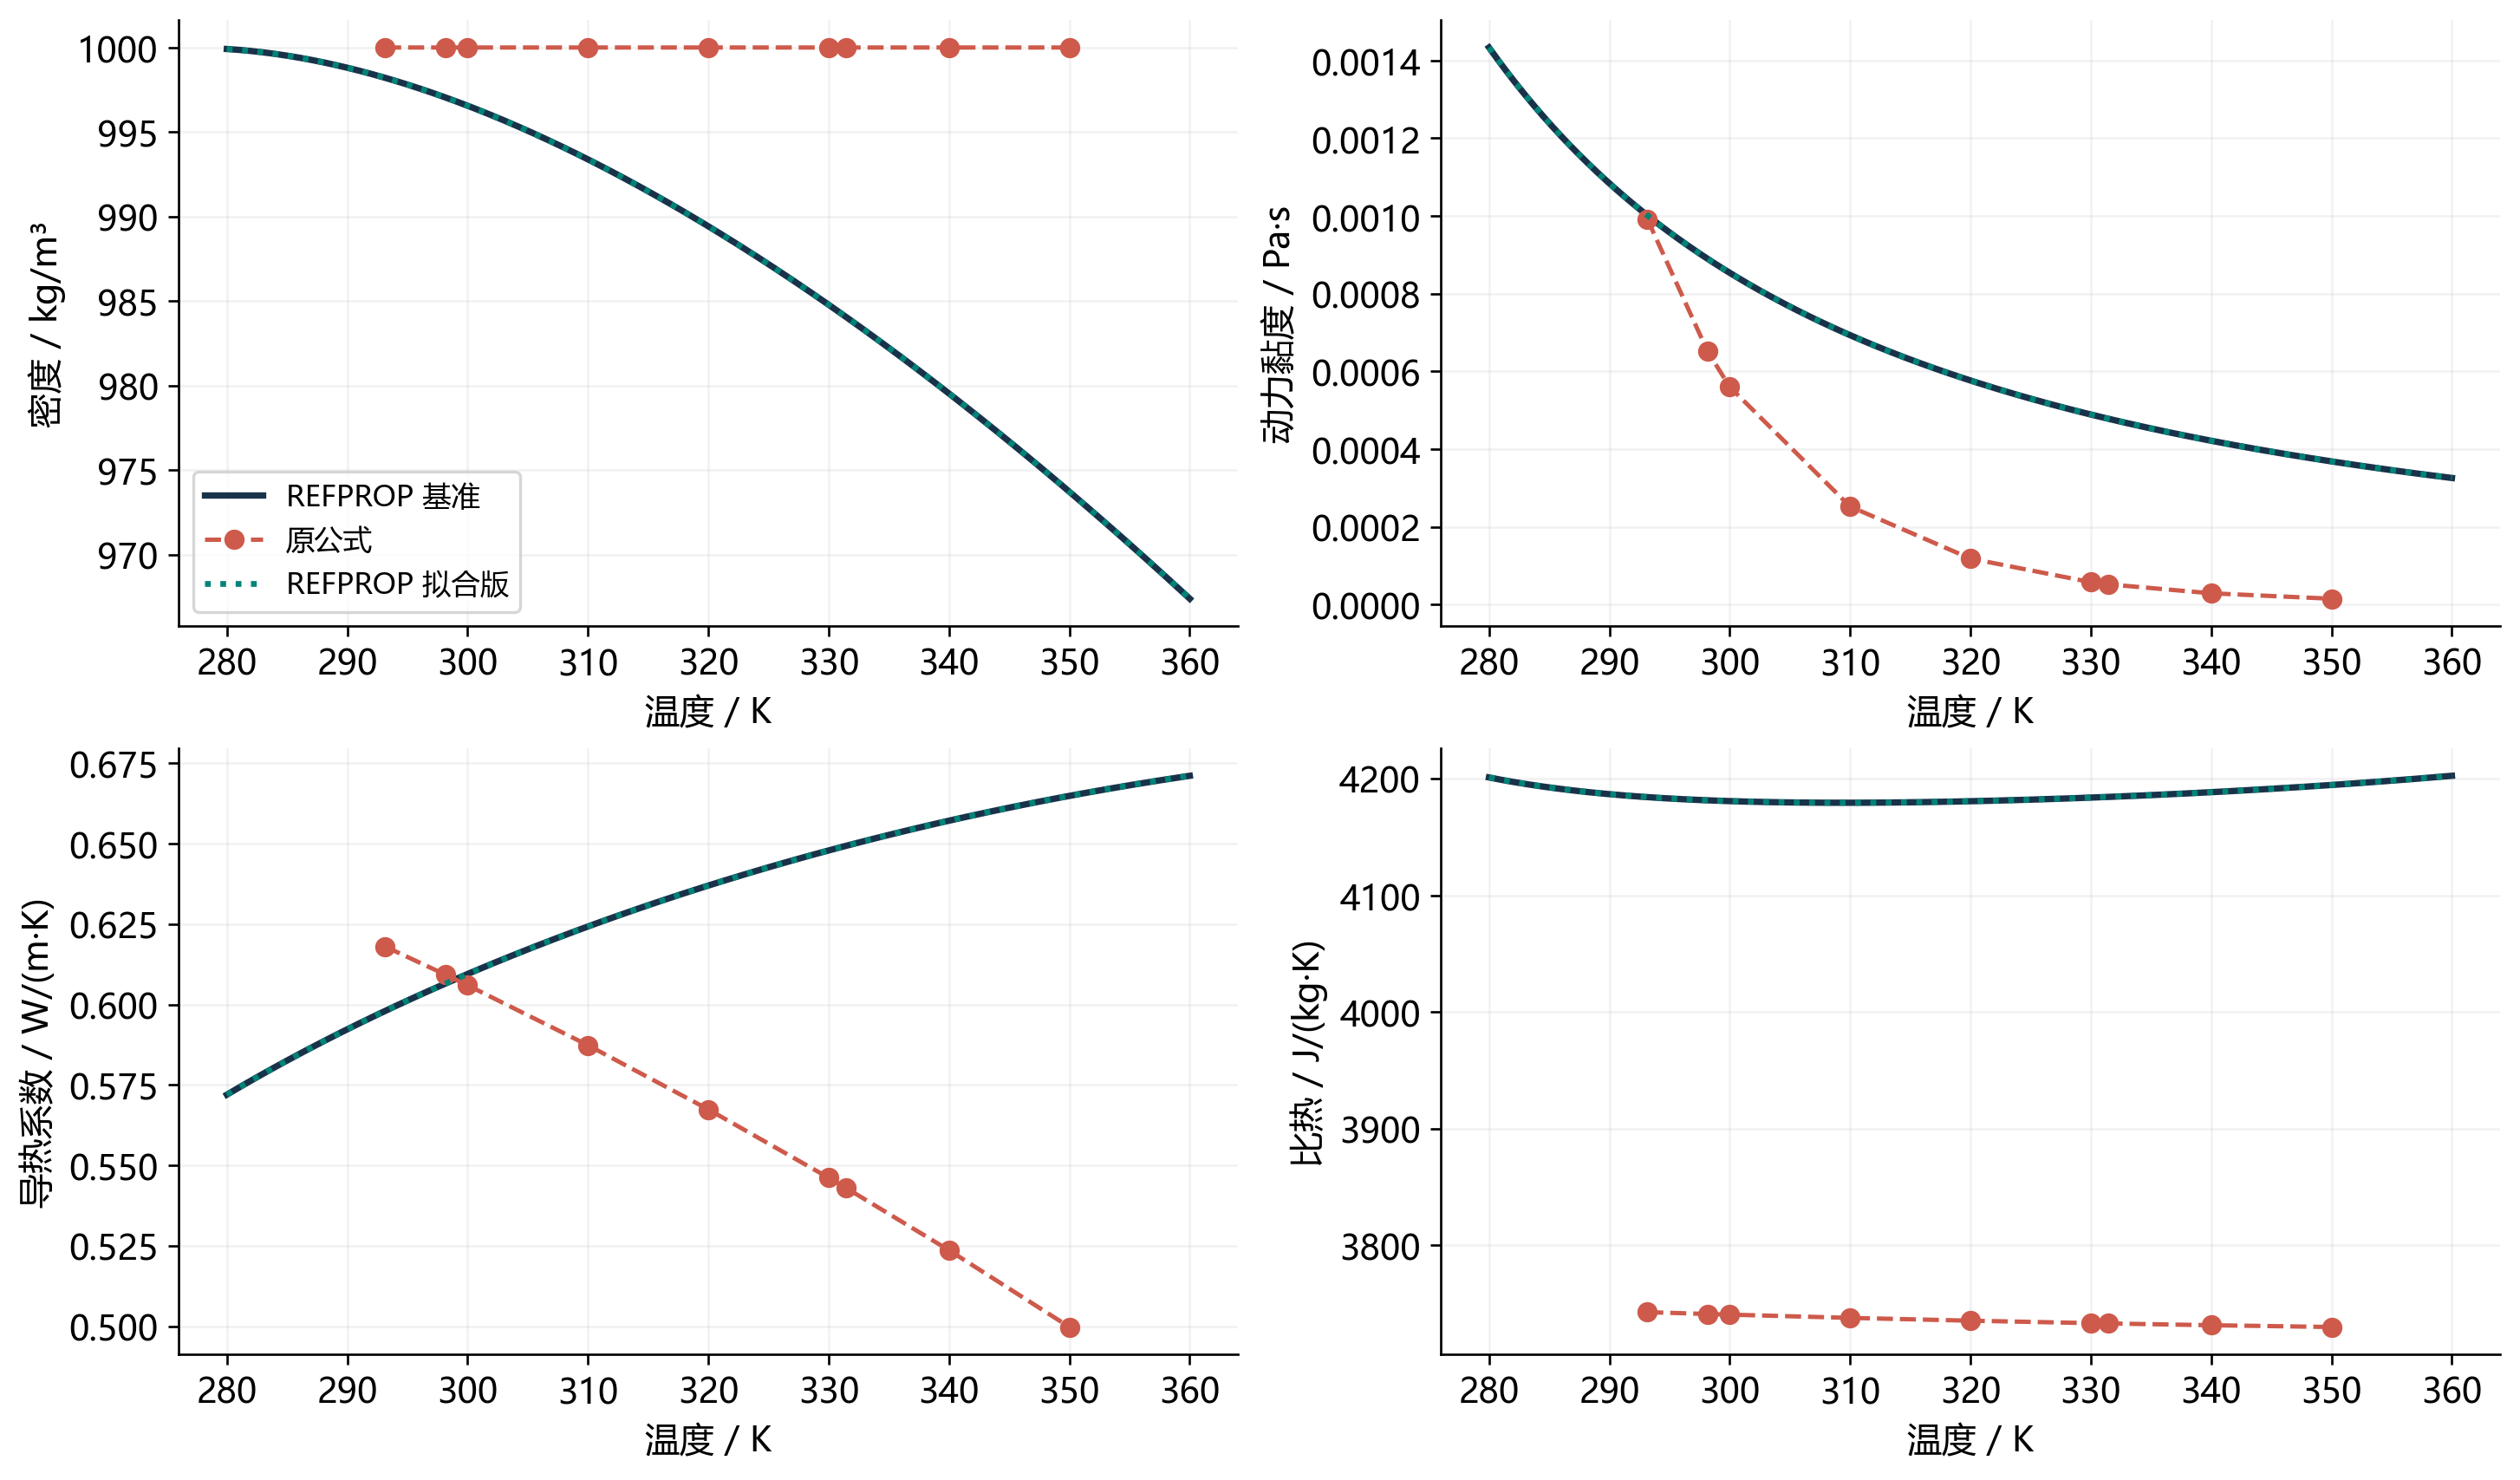
\includegraphics[width=\linewidth]{../../figs/midterm_asset_udf_01_四项物性温度曲线.png}
\caption{四项水物性随温度的变化：参考、原公式与最终REFPROP拟合版。排查候选公式与最终拟合版分别保留，不混用。}\label{fig:udf-curves}
\end{figure}
\clearpage
\setcounter{figure}{3}
\begin{figure}[htbp]\centering
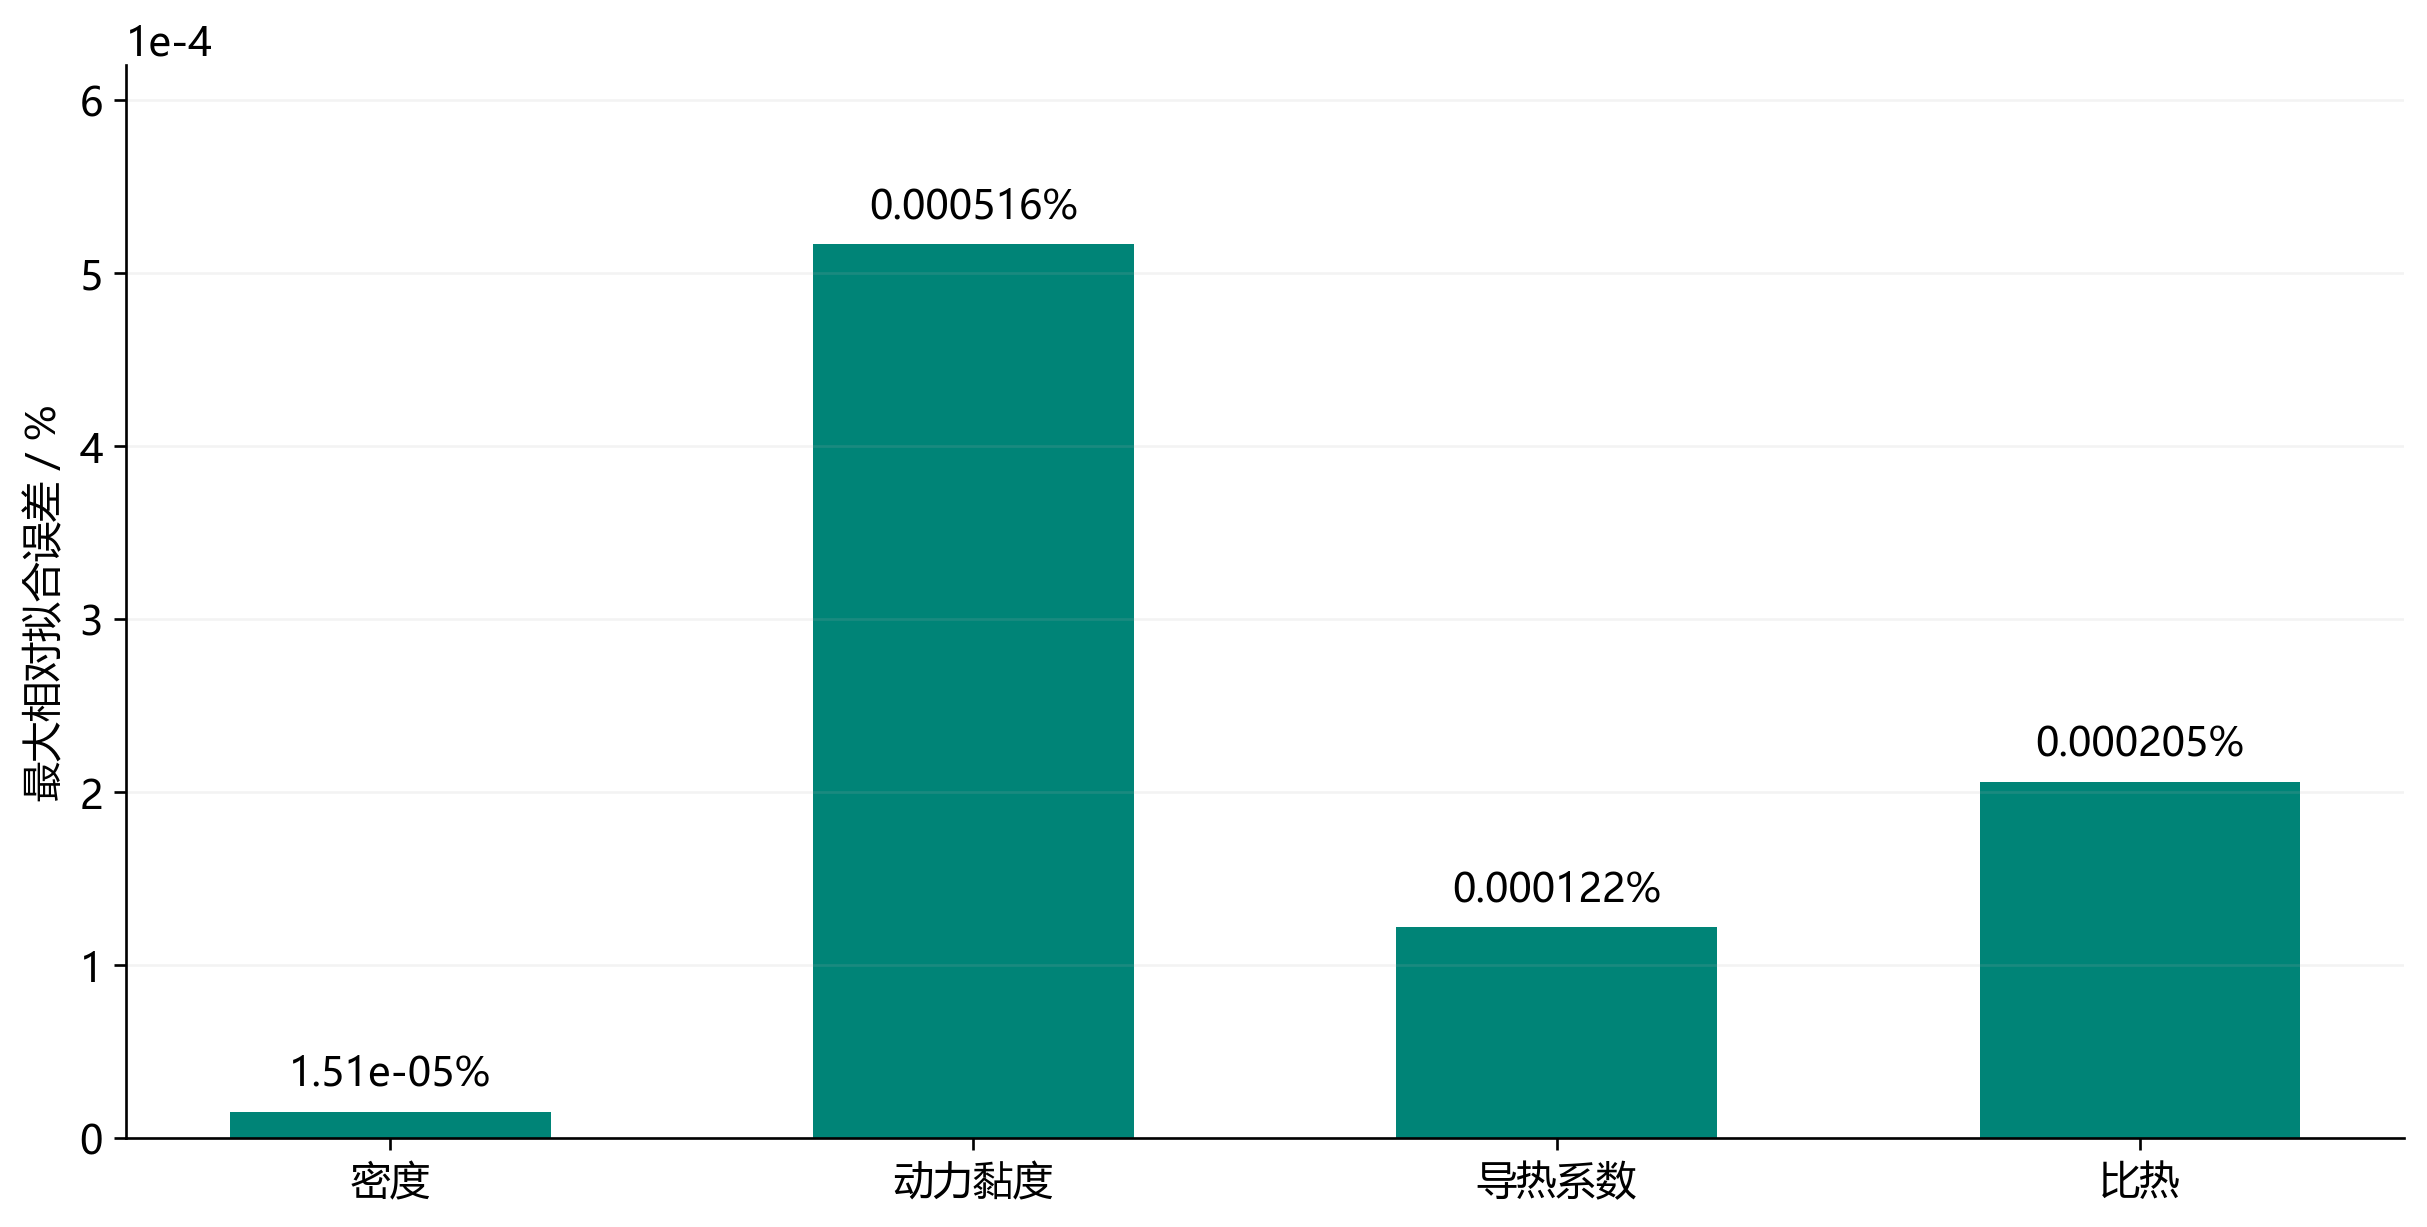
\includegraphics[width=\linewidth]{../../figs/midterm_asset_udf_03_1601点拟合误差.png}
\caption{1601温度点核对记录中的四项最大相对拟合误差。}\label{fig:udf-fit-error}
\end{figure}
\clearpage
\setcounter{figure}{4}
\begin{figure}[htbp]\centering
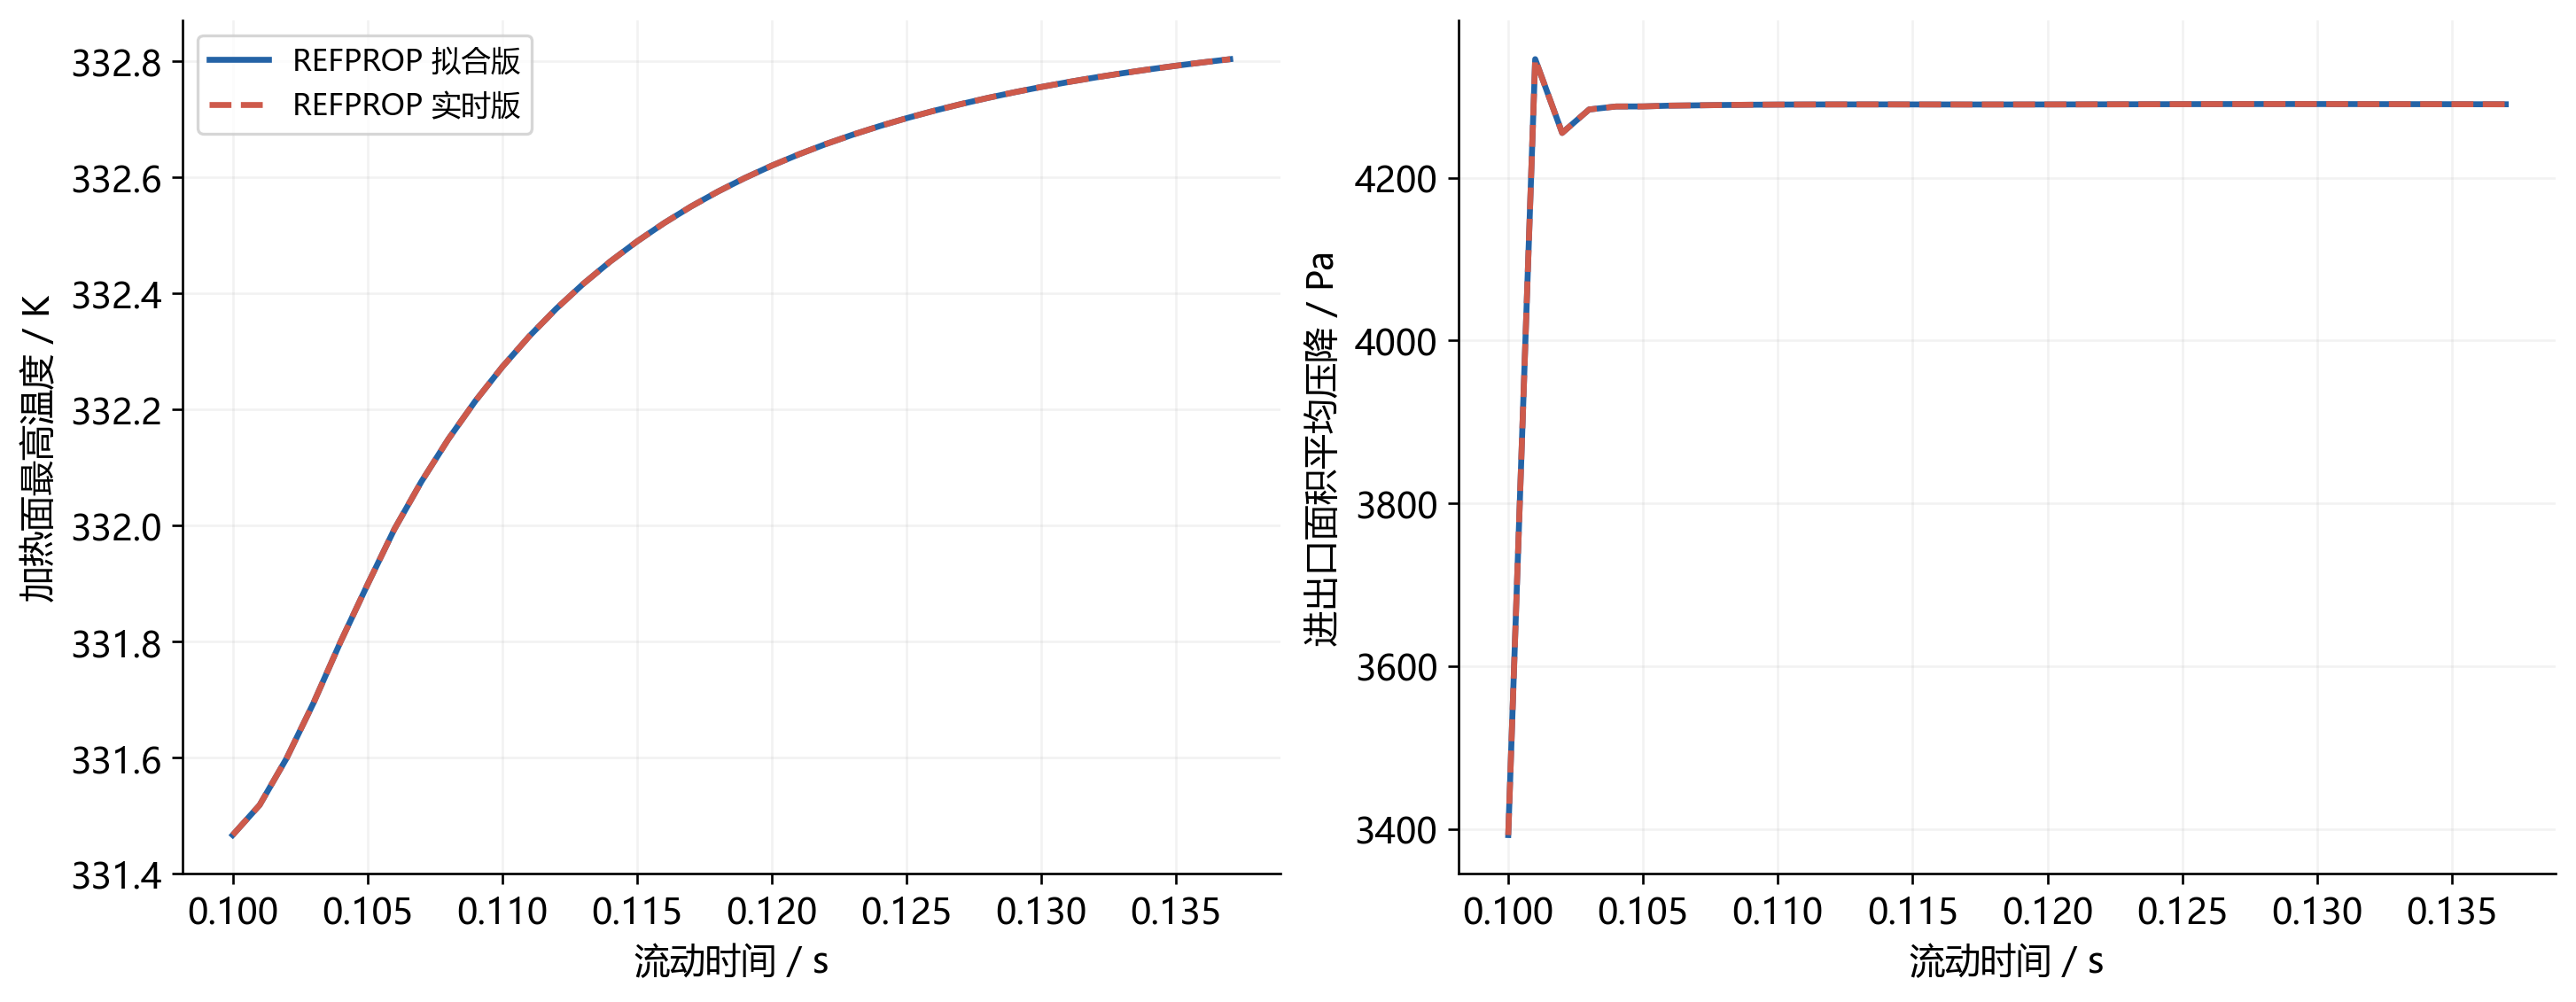
\includegraphics[width=\linewidth]{../../figs/midterm_asset_udf_04_同一时段求解结果.png}
\caption{相同初场和时间步下两种物性实现的共同时间段对照。}\label{fig:udf-common}
\end{figure}
\clearpage
\setcounter{figure}{5}
\begin{figure}[htbp]\centering
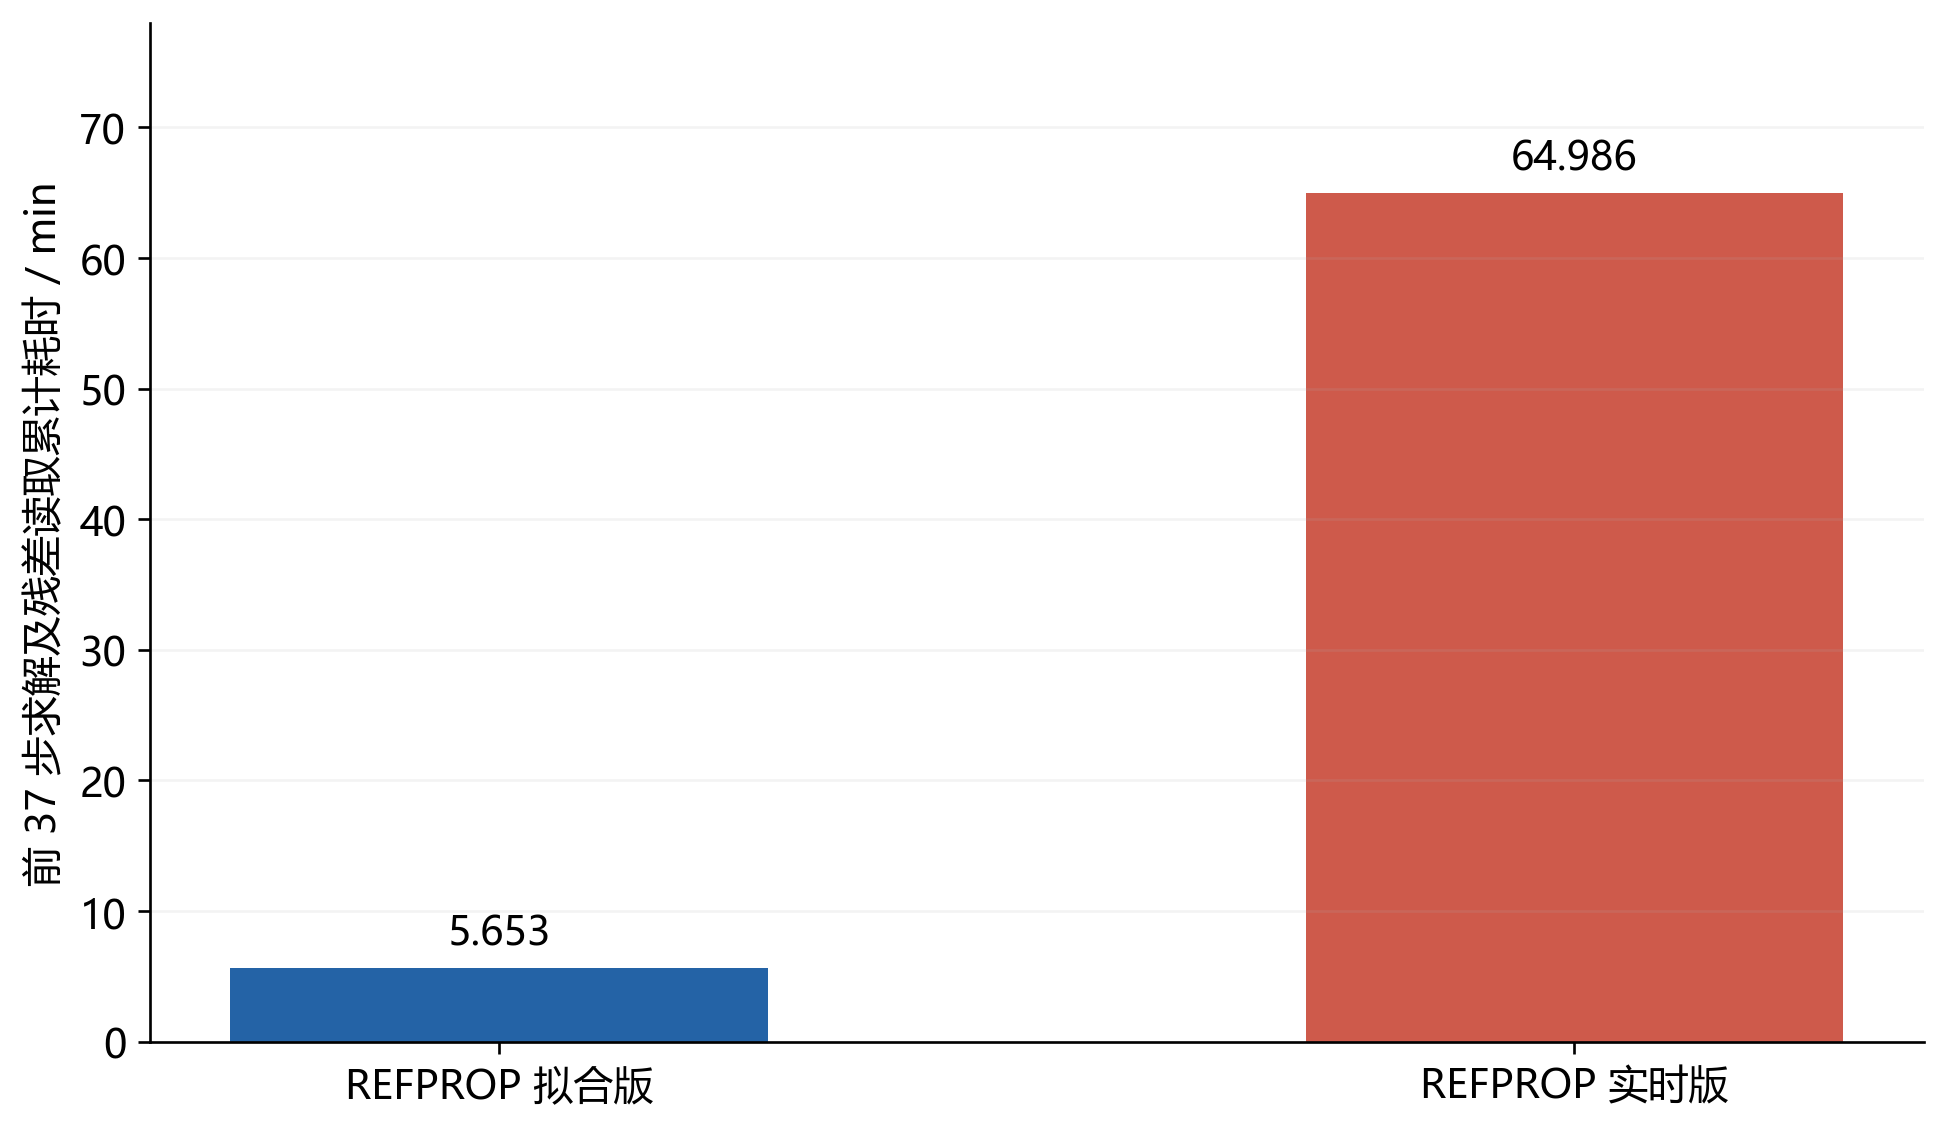
\includegraphics[width=.8\linewidth]{../../figs/midterm_asset_udf_05_共同37步计算耗时.png}
\caption{共同前37步的求解及残差读取耗时；不是不同总步数或代理模型的加速比较。}\label{fig:udf-time}
\end{figure}
\clearpage
\setcounter{table}{3}
\begin{table}[H]\centering
\caption{NACA2416 在 $0.2\,\mathrm{s}$ 的七档网格结果}
\label{tab:mesh}
\begin{tabular*}{\textwidth}{@{\extracolsep{\fill}}rrrr@{}}\toprule
\rowcolor{ydzjlight} 单元数 / 万 & $\overline T$ / K & $T_{\max}$ / K & $\Delta p$ / Pa \\
\midrule
26.02 & 304.6684 & 344.6755 & 2505.204 \\
57.51 & 304.4113 & 345.2657 & 2389.274 \\
107.36 & 303.9449 & 345.1536 & 2440.766 \\
152.49 & 305.0933 & 346.0488 & 2389.938 \\
294.33 & 304.3736 & 345.9640 & 2355.838 \\
323.51 & 304.3009 & 345.9838 & 2348.320 \\
461.08 & 305.9860 & 346.6188 & 2448.714 \\
\bottomrule\end{tabular*}\end{table}
\clearpage
\setcounter{figure}{6}
\begin{figure}[H]\centering
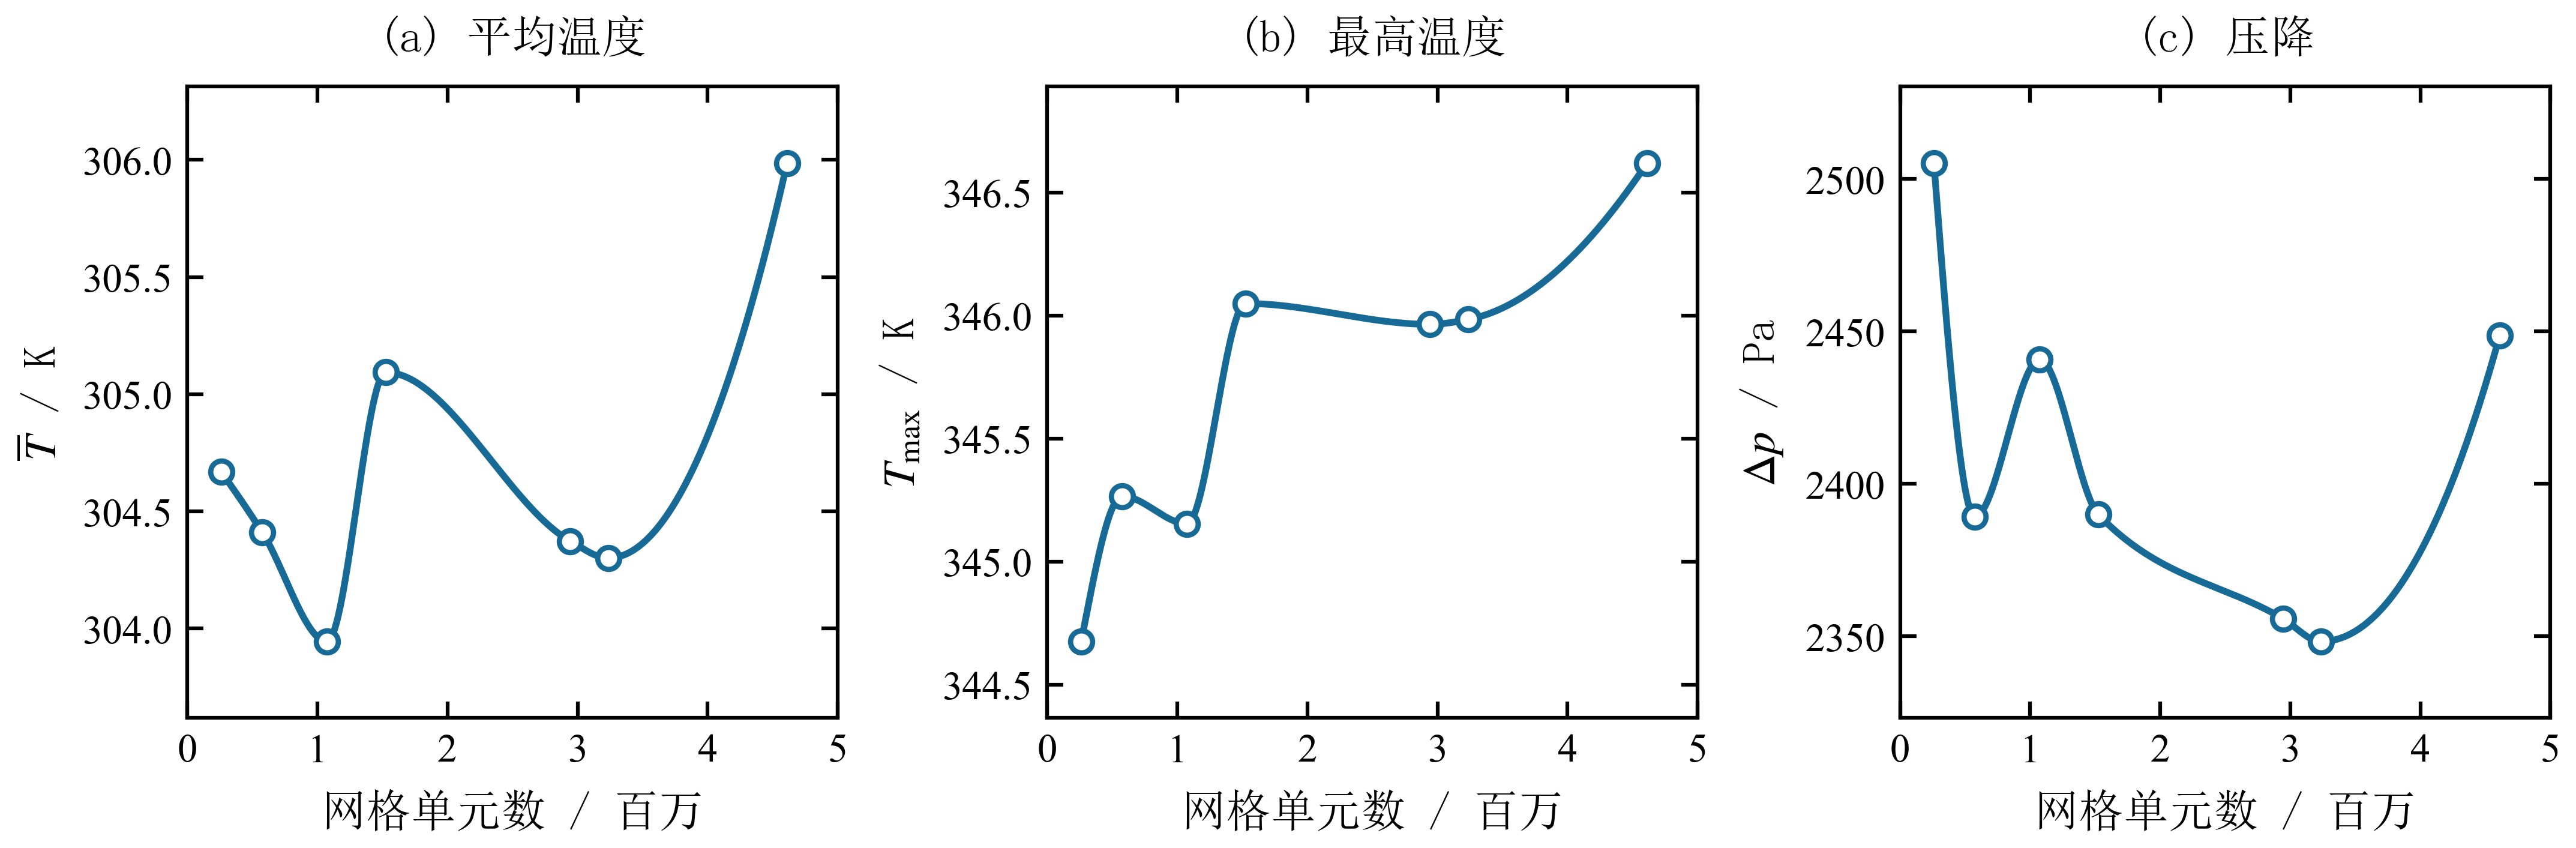
\includegraphics[width=\textwidth]{../../figs/month3_mesh_temperature_pressure.png}
\caption{七档网格的平均温度、最高温度与静压差原始值}
\label{fig:month3_mesh}\end{figure}
\clearpage
\setcounter{table}{4}
\begin{table}[H]\centering
\caption{以323万档为参考的温度与压降相对差异（\%）}
\label{tab:mesh_ref323}
\begin{tabular*}{\textwidth}{@{\extracolsep{\fill}}rrrr@{}}\toprule
\rowcolor{ydzjlight} 单元数 / 万 & 平均温度差异 & 最高温度差异 & 压降差异 \\
\midrule
26.02 & 0.1208 & 0.3782 & 6.6807 \\
57.51 & 0.0363 & 0.2076 & 1.7440 \\
107.36 & 0.1170 & 0.2400 & 3.9367 \\
152.49 & 0.2604 & 0.0188 & 1.7722 \\
294.33 & 0.0239 & 0.0057 & 0.3201 \\
323.51 & 0.0000 & 0.0000 & 0.0000 \\
461.08 & 0.5537 & 0.1835 & 4.2751 \\
\bottomrule\end{tabular*}\end{table}
\clearpage
\setcounter{figure}{7}
\begin{figure}[H]\centering
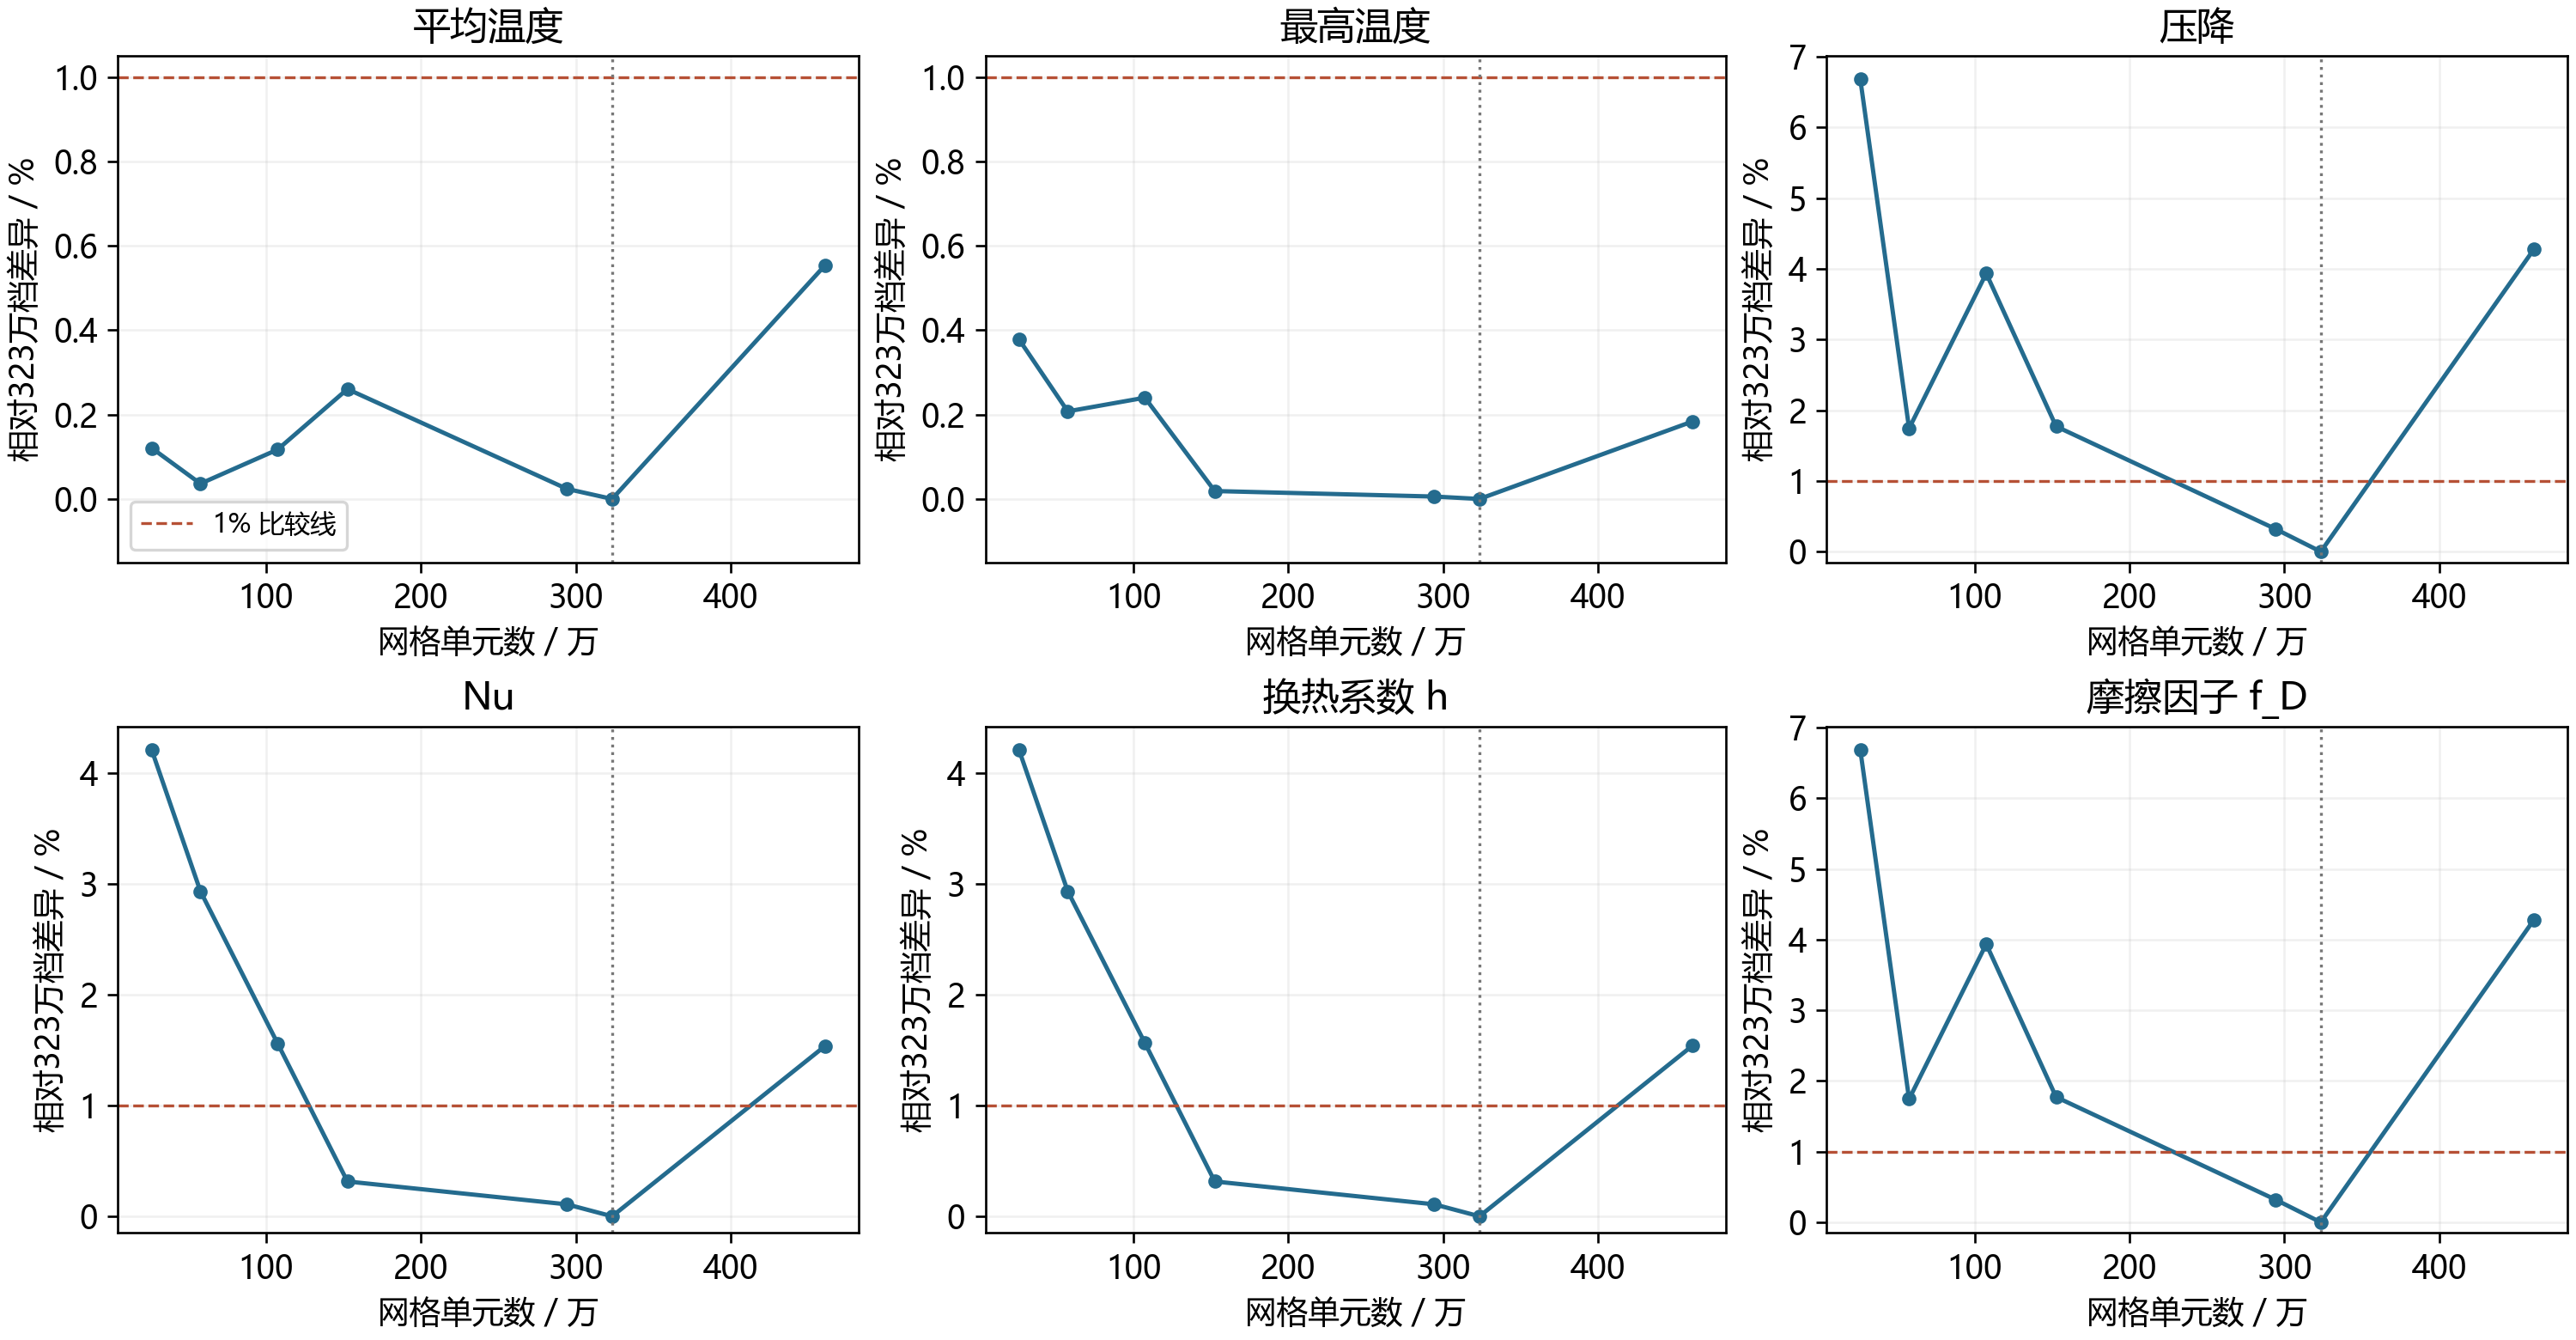
\includegraphics[width=0.98\textwidth]{../../figs/month3_mesh_errors_ref323.png}
\caption{各指标统一以323万档为参考的相对差异；虚线为 $1\%$ 比较线}
\label{fig:month3_errors323}\end{figure}
\clearpage
\setcounter{figure}{8}
\begin{figure}[H]\centering
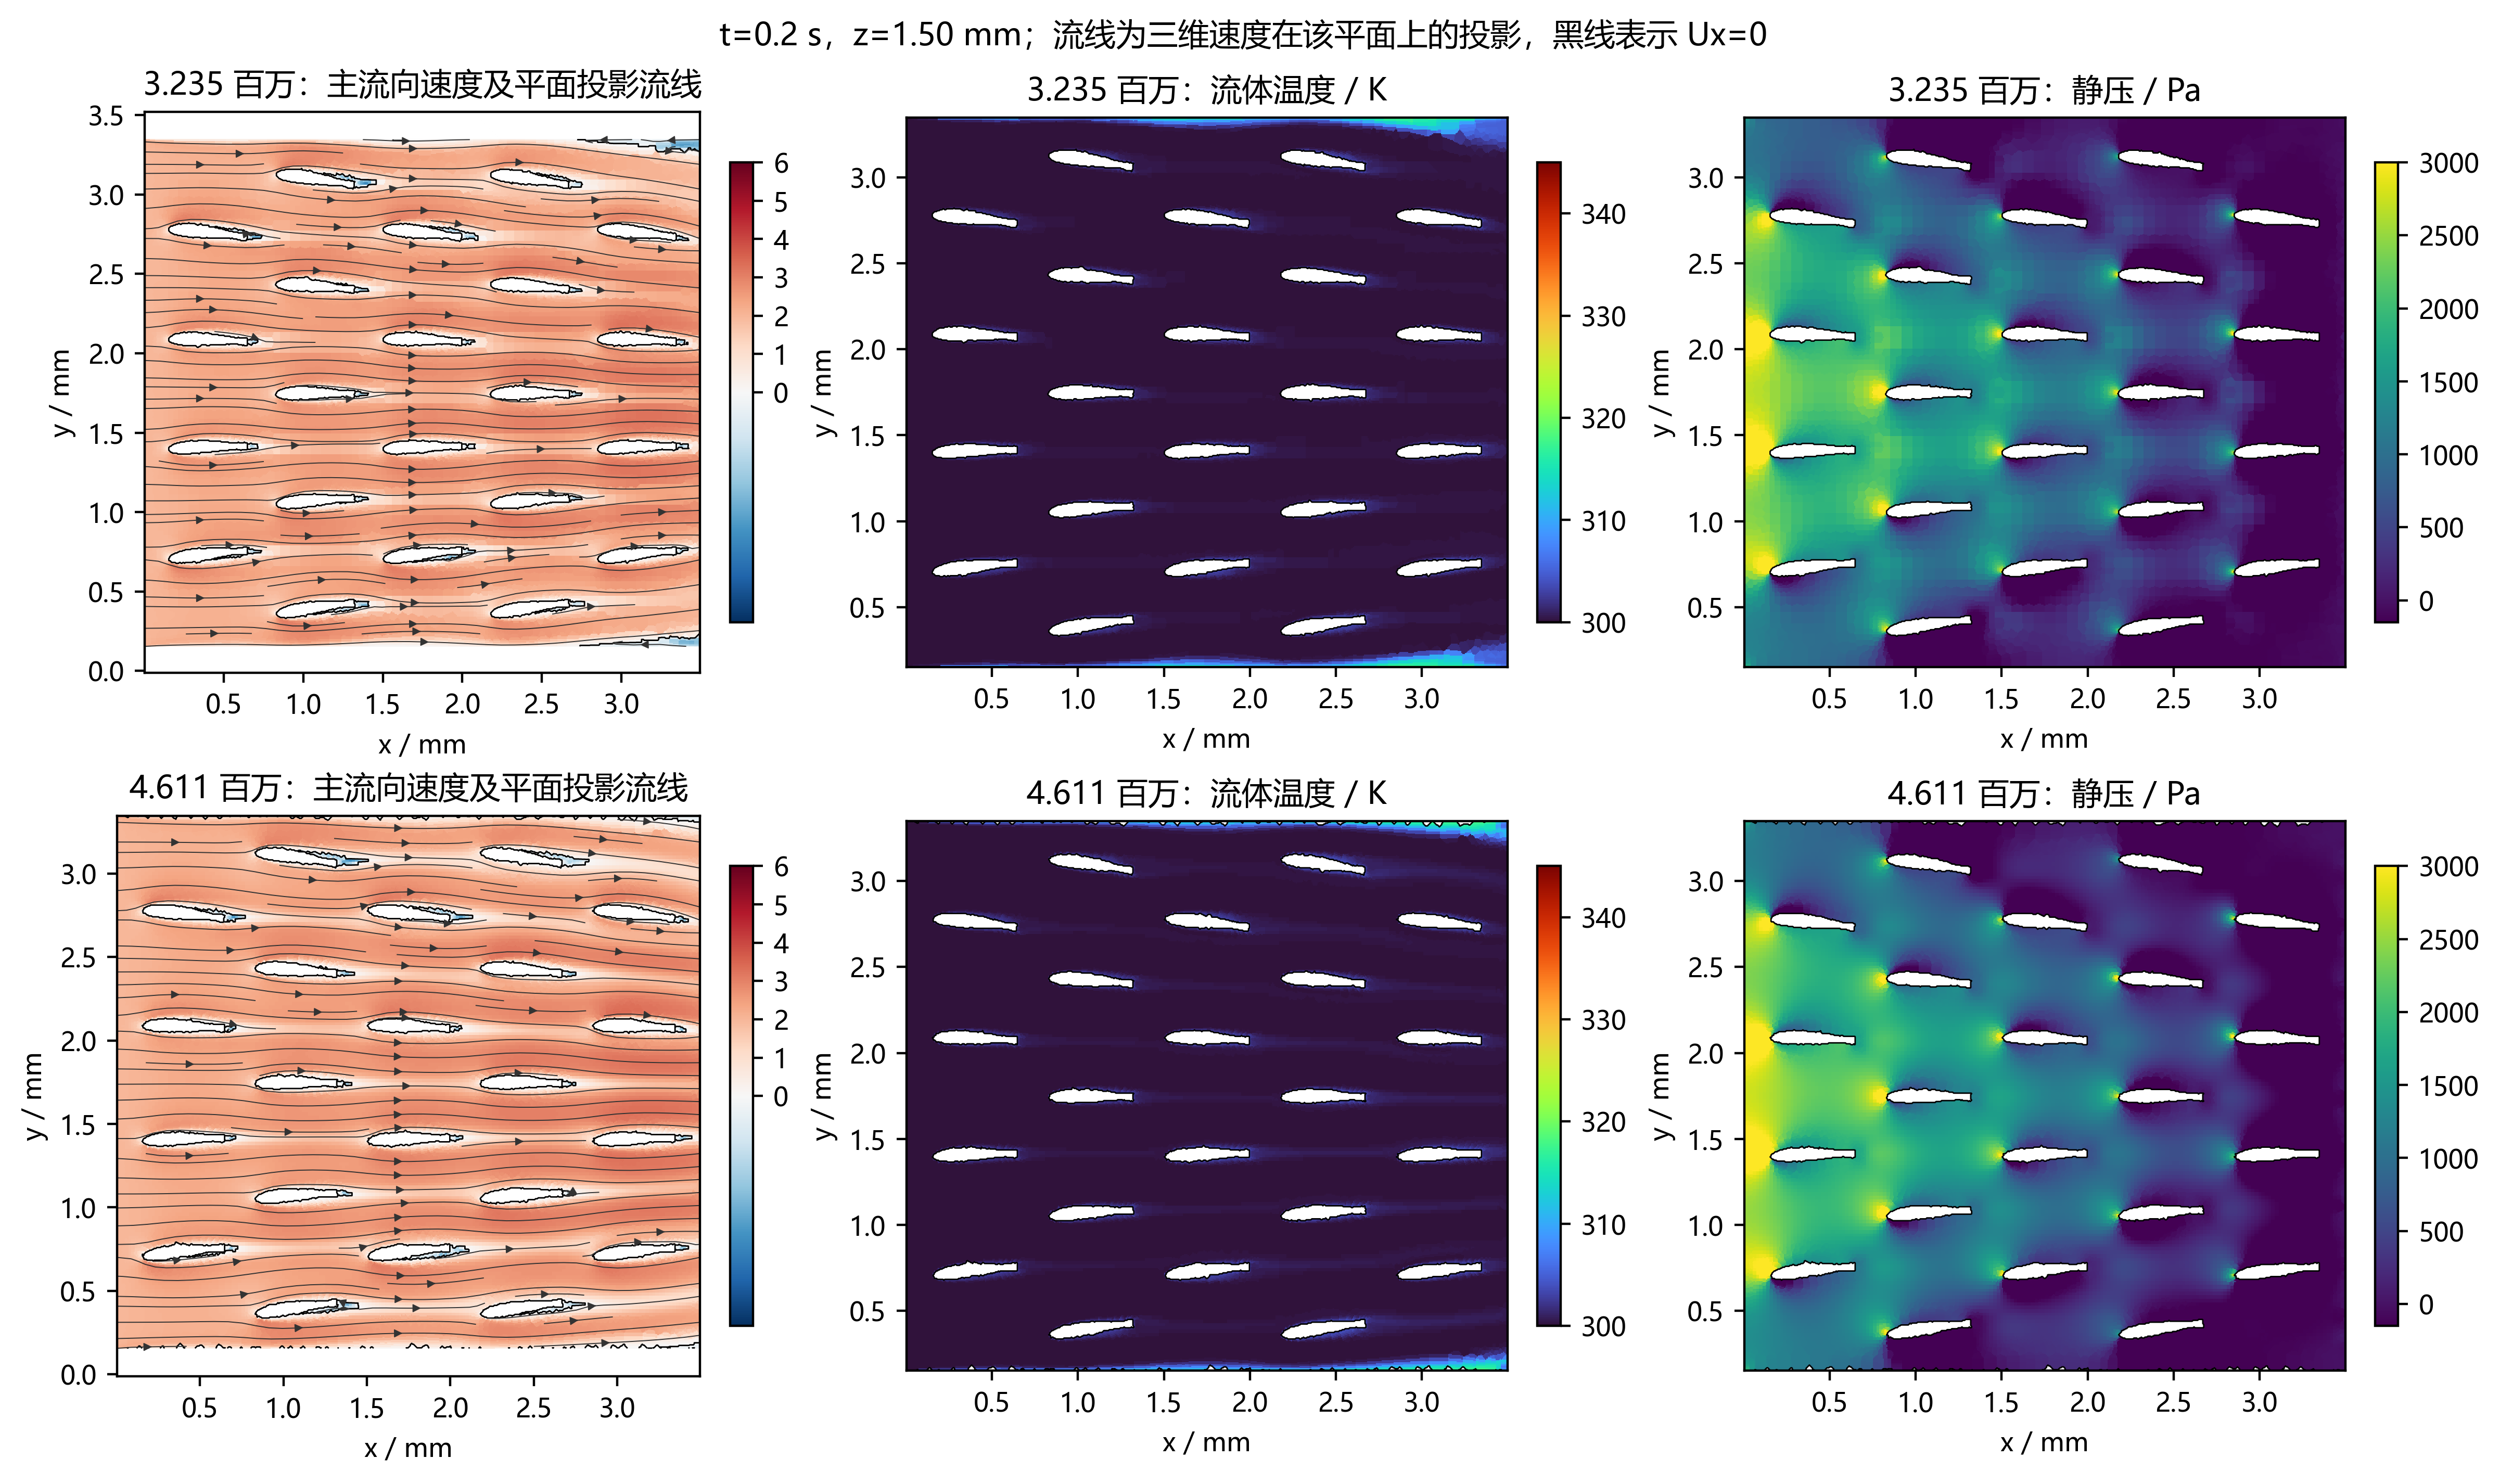
\includegraphics[width=\textwidth]{../../figs/month3_mesh_flowfield.png}
\caption{以323万档（上排）为参照的中高平面流动场对比；下排为461万档，$t=0.2\,\mathrm{s}$}
\label{fig:month3_flowfield}\end{figure}
\clearpage
\setcounter{figure}{9}
\begin{figure}[H]\centering
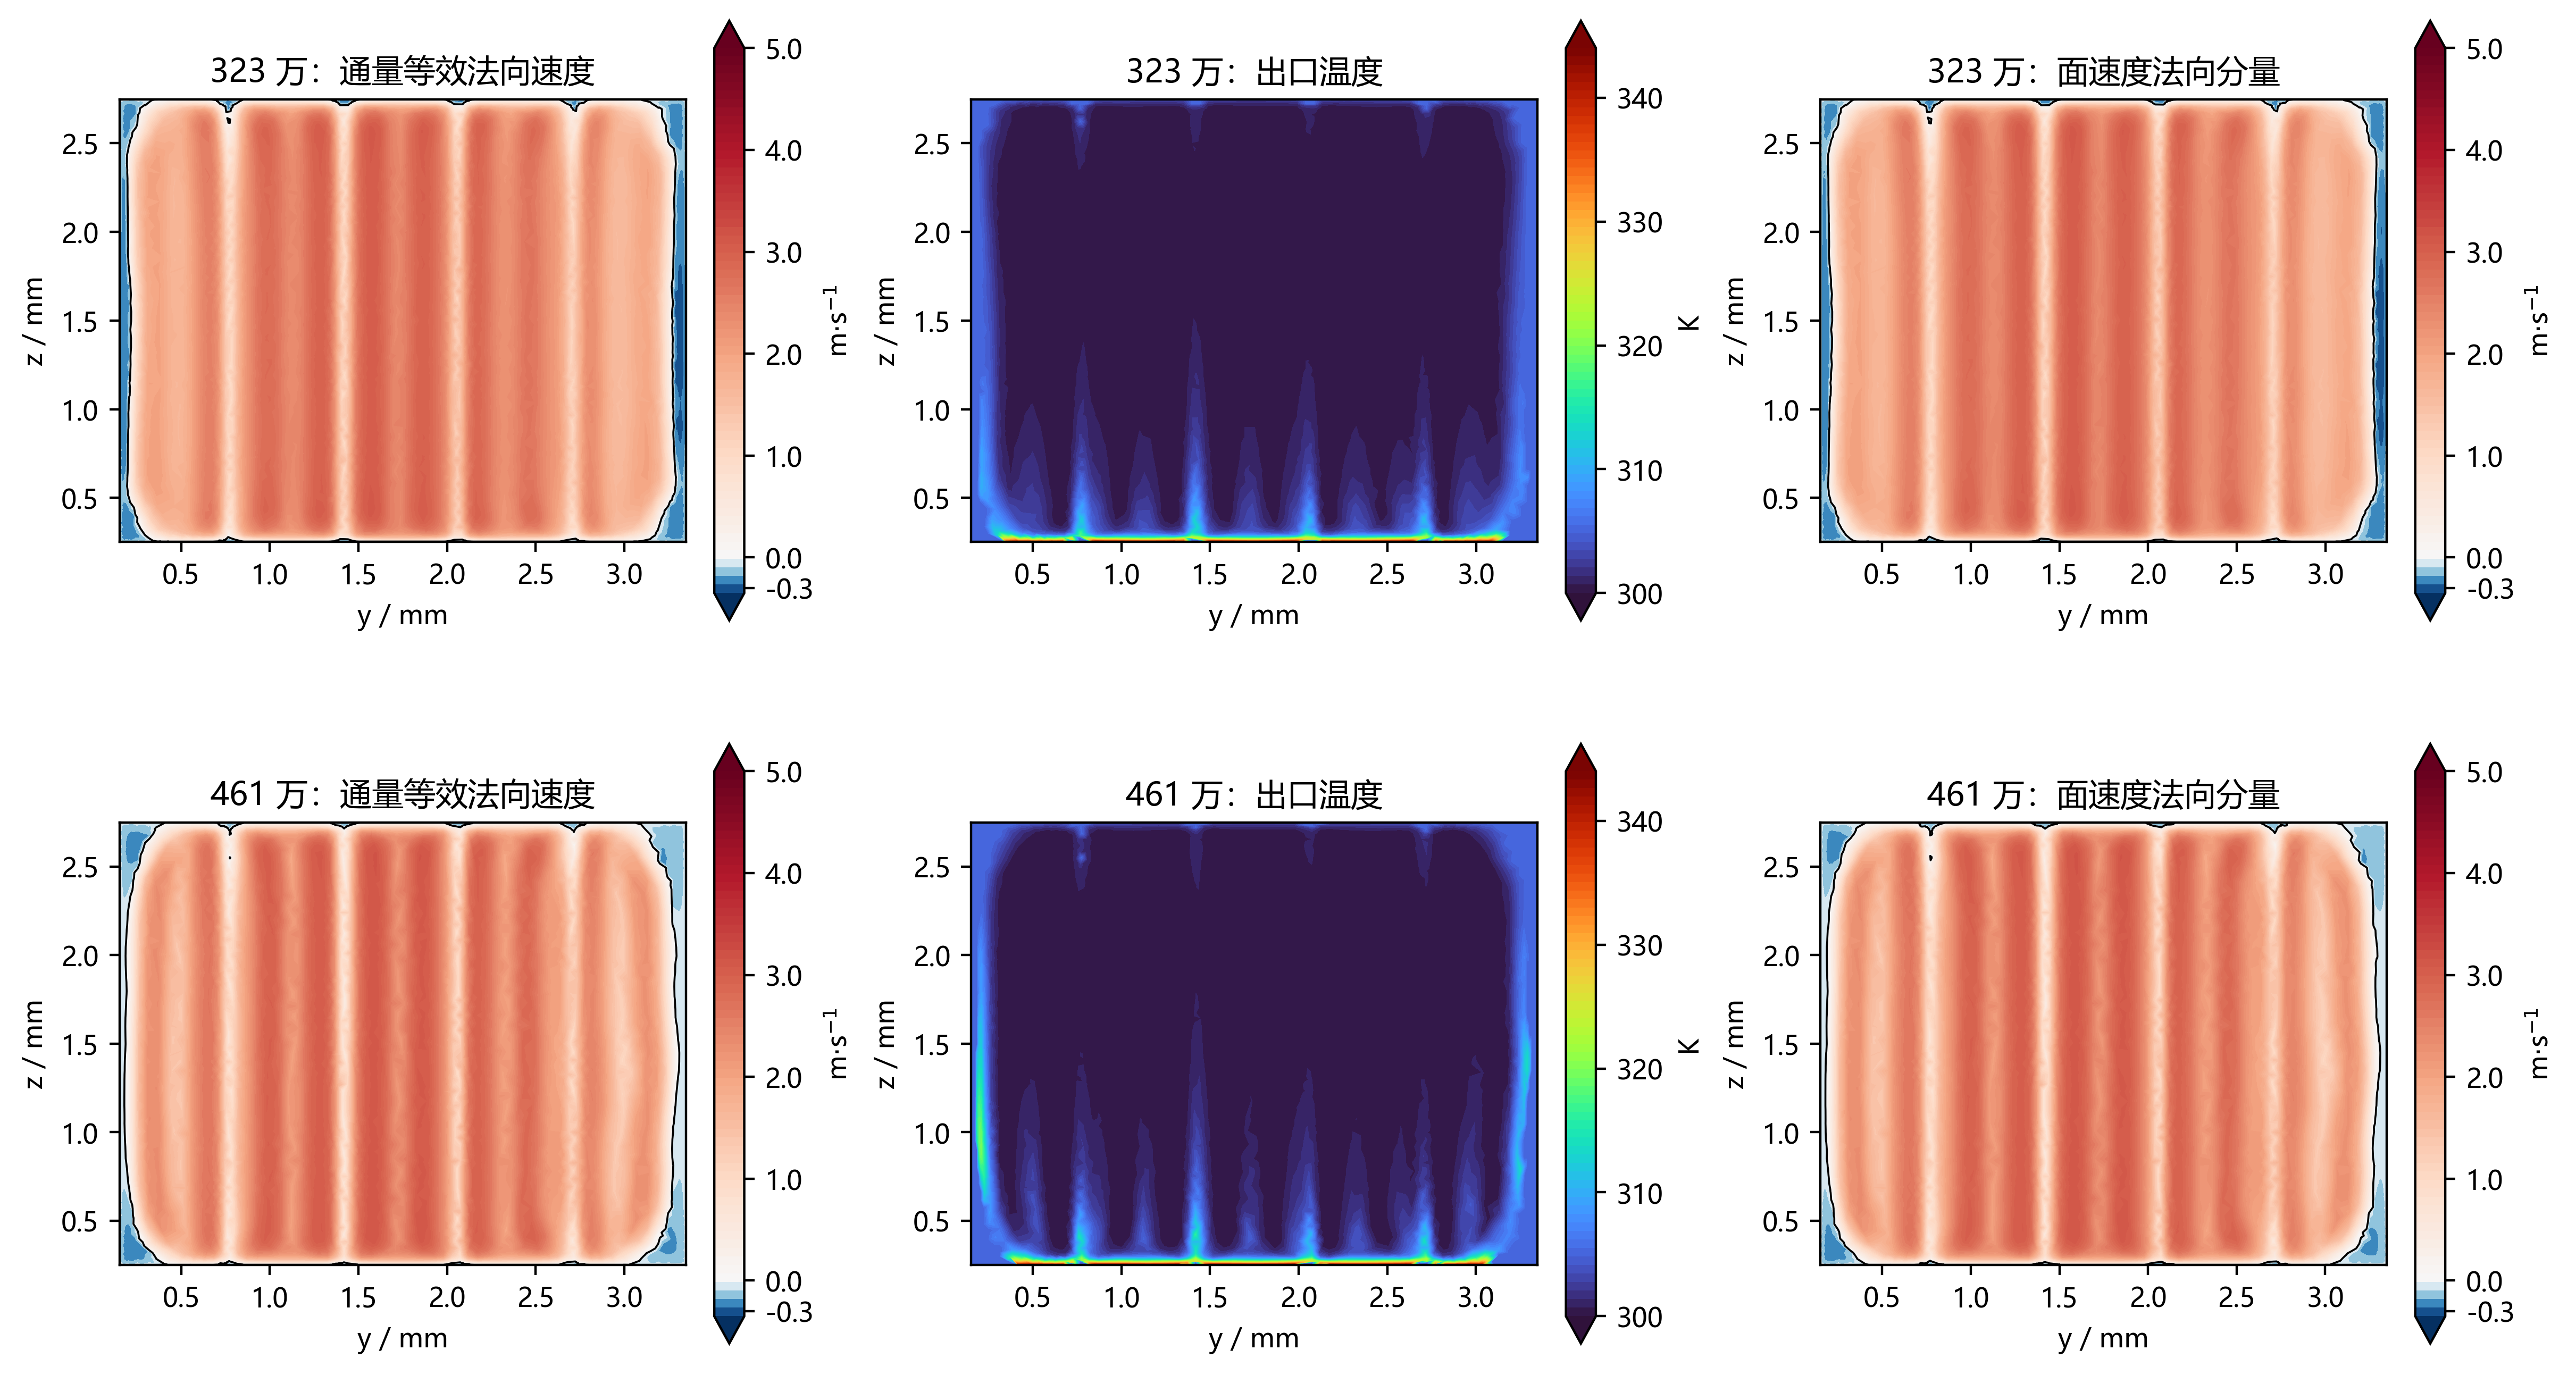
\includegraphics[width=\textwidth]{../../figs/month3_mesh_outlet.png}
\caption{以323万档（上排）为参照的出口速度与温度对比；下排为461万档}
\label{fig:month3_outlet}\end{figure}
\clearpage
\setcounter{figure}{10}
\begin{figure}[H]\centering
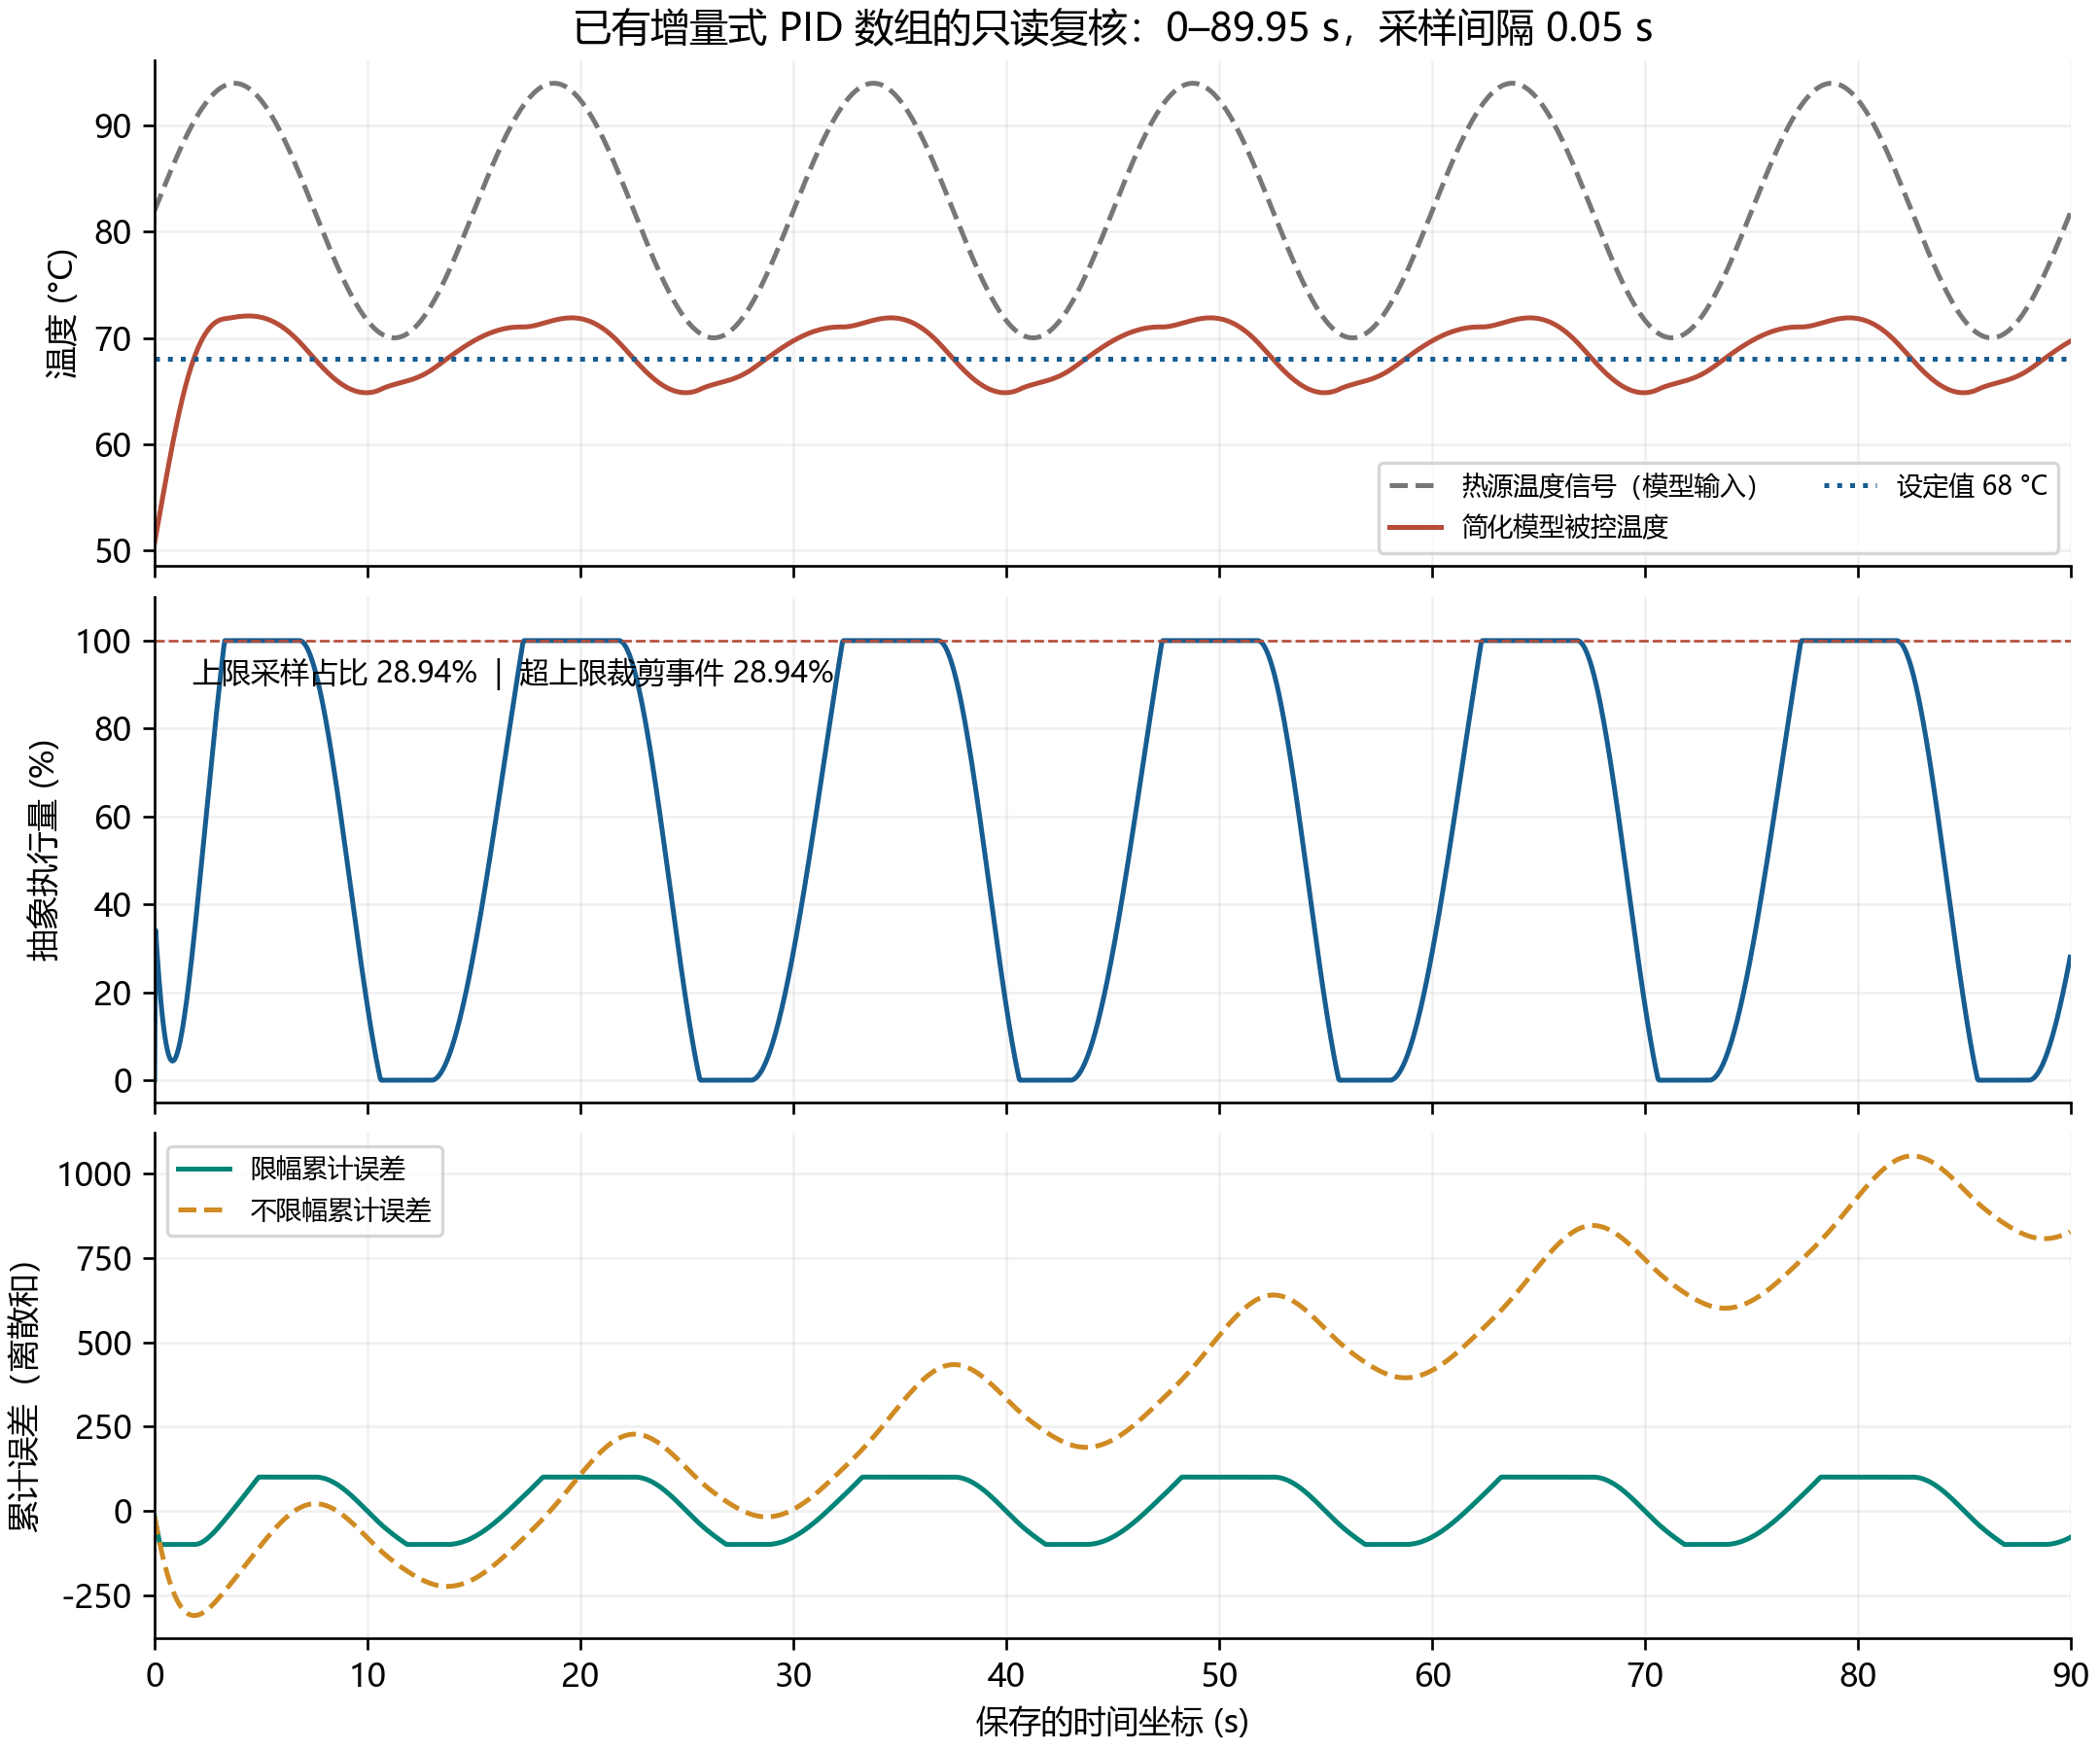
\includegraphics[width=.9\linewidth,height=150mm,keepaspectratio]{../../figs/midterm_asset_pid_verified.png}
\caption{已有简化 PID 温控数组的只读复核。上图为温度扰动与被控温度，中图为限幅执行量，下图为开关累计误差限幅时的累计值；不表示实物流量。}\label{fig:20}
\end{figure}
\clearpage
\setcounter{table}{5}
\begin{table}[H]\centering\small
\caption{保存 PID 时序的工况与复核指标}\label{tab:11}
\begin{tabularx}{\linewidth}{@{}Y Y Y@{}}\toprule
\rowcolor{ydzjlight} 项目 & 数值或状态 & 统计与适用范围 \\\midrule
设定值／初始温度 & 68／50 $^\circ$C & 首个保存温度为更新后50.67625 $^\circ$C。\\
离散增益／采样周期 & $K_p=8.0,K_i=0.5,K_d=2.0$；0.05 s & 增量更新的已有参数，不直接等同连续增益。\\
全时段温度范围 & 50.6763--72.0657 $^\circ$C & 相对68 $^\circ$C全时段最大偏高4.0657 K。\\
后半时段峰值偏高 & 3.8865 K & 月报3.9 K对应后半段45--89.95 s，不是全程峰值。\\
执行量范围与均值 & 0--100\%；均值54.3705\% & 为经验模型抽象动作，未标定为泵速或流量。\\
上限采样占比 & 28.9444\% & 以保存数组 $U\ge100-10^{-10}$ 逐点统计；月报29.3\%未由当前数组复现。\\
累计误差峰值 & 限幅100；不限幅1052.6016 & 仅记录累计量变化，不能单独证明抗饱和有效。\\
开关限幅后的温度／执行量差 & 两者最大绝对差均为0 & 当前程序没有将该累计量用于增量更新。\\
\bottomrule\end{tabularx}\end{table}
\clearpage
\setcounter{table}{6}
\begin{table}[H]\centering
\caption{本月工作与材料状态}\label{tab:tasks}
\begin{tabularx}{\textwidth}{@{}Y Y Y@{}}
\toprule
\rowcolor{ydzjlight} 工作 & 状态 & 依据或缺口 \\
\midrule
翼型专题研究 & 已有历史结果 & 六种翼型基准及13条小模型分支，不等于完整参数矩阵 \\
翼型参数分组 & 方案待落实 & 本稿列出建议设计；完整数据尚未提供 \\
UDF 修改及对照 & 已有代表记录 & 1601点拟合与共同0.137 s实现对照 \\
网格检验 & 阶段分析 & 323万档作参考，联合收敛仍待复核 \\
PID 数学模拟 & 已有时序 & 1800点保存数据；抗饱和实现存在待修问题 \\
\bottomrule\end{tabularx}\end{table}
\clearpage
\setcounter{table}{7}
\begin{table}[H]\centering
\caption{后续工作及所需产出}\label{tab:plan}
\begin{tabularx}{\textwidth}{@{}Y Y Y@{}}
\toprule
\rowcolor{ydzjlight} 工作 & 状态  \\
\midrule
小块适用分界线 & 热流密度与小块选择的条件化关系 \\
流道几何形态的优化 & 统一定义和对照数据  \\
翼型代理模型的 XGBoost 尝试 & 先补分组数据再训练和独立测试  \\
\bottomrule\end{tabularx}\end{table}
\clearpage
\begin{thebibliography}{9}

\bibitem{smallmodels} 小模型保存结果与性能汇总. 项目仿真资料, 2026. 见配套数据文件 small\_model\_results.csv 及 model\_sources.json；数值由 Case／Data 提取，图像由实际面元及表面温度生成。
\bibitem{airfoil} 微通道液冷场景下的翼型参数. 项目资料, 2026.
\bibitem{control} 控制理论与 PID 算法相关资料. 项目资料, 2026.

% ---------- 控制理论学习书籍（张昊洋补充）----------
\bibitem{hushousong} 胡寿松. 自动控制原理[M]. 8 版. 北京: 科学出版社, 2023.
\bibitem{astrom} {\AA}STR{\"O}M K J, H{\"A}GGLUND T. PID Controllers: Theory, Design, and Tuning[M]. 2nd ed. Research Triangle Park: Instrument Society of America, 1995.
\bibitem{franklin} FRANKLIN G F, POWELL J D, EMAMI-NAEINI A. Feedback Control of Dynamic Systems[M]. 8th ed. London: Pearson, 2019.
\bibitem{ogata} OGATA K. Modern Control Engineering[M]. 5th ed. London: Pearson, 2010.
\bibitem{brunton} BRUNTON S L, KUTZ J N. Data-Driven Science and Engineering: Machine Learning, Dynamical Systems, and Control[M]. 2nd ed. Cambridge: Cambridge University Press, 2022.
\end{thebibliography}
\end{document}
